\documentclass[
   paper=a4,
   twoside=false,
   parskip=half,
   listof=entryprefix,
   listof=totoc,
   index=totoc,
   bibliography=totoc,
   headsepline,
]{scrbook}

\usepackage{silence}
\WarningFilter{biblatex}{File 'ngerman-iso.lbx'}
\WarningFilter{biblatex}{'\mainlang'}
\WarningFilter{biblatex}{Bibliography string 'online' untranslated}
\WarningFilter{hyperref}{Token not allowed in a PDF string}

%%%%%%%%%%%%%%%%%%%%%%%%%%%%%%%%%%%%%%%%%%%%%%%%%%%%%%%%%%%%%%%%%%%%%%%%%%%%%%
% Fonts Fonts Fonts
%%%%%%%%%%%%%%%%%%%%%%%%%%%%%%%%%%%%%%%%%%%%%%%%%%%%%%%%%%%%%%%%%%%%%%%%%%%%%%
\usepackage[utf8]{inputenc}
\usepackage[ngerman]{babel}
\usepackage[T1]{fontenc}
\usepackage{scrhack}
\usepackage{pdfpages,graphicx,subcaption,lastpage,xspace}
\graphicspath{ {./images} }
\usepackage{float,xcolor,colortbl,csquotes,microtype,etoolbox}
\MakeOuterQuote{"}
\usepackage[automark,markcase=ignoreuppercase,autooneside=false]{scrlayer-scrpage}
\usepackage[official]{eurosym}
\usepackage[breaklinks,colorlinks,linkcolor=black,citecolor=black,filecolor=black,urlcolor=black]{hyperref}

%Requiers Incscape to be installed%
\usepackage[inkscapeformat=png,inkscapedpi=600]{svg}
% Used for Tables spanning across Pages %
\usepackage{longtable}

%%%%%%%%%%%%%%%%%%%%%%%%%%%%%%%%%%%%%%%%%%%%%%%%%%%%%%%%%%%%%%%%%%%%%%%%%%%%%%
% Listings Paket
%%%%%%%%%%%%%%%%%%%%%%%%%%%%%%%%%%%%%%%%%%%%%%%%%%%%%%%%%%%%%%%%%%%%%%%%%%%%%%
\usepackage{listings,caption,pmboxdraw}
\definecolor{codebg}{rgb}{0.95,0.95,0.95}
\definecolor{lightgray}{rgb}{.9,.9,.9}
\definecolor{darkgray}{rgb}{.4,.4,.4}
\definecolor{purple}{rgb}{0.65, 0.12, 0.82}

\lstdefinelanguage{JavaScript}{
  keywords={break, case, catch, continue, debugger, default, delete, do, else, false, finally, for, function, if, in, instanceof, new, null, return, switch, this, throw, true, try, typeof, var, void, while, with, const},
  morecomment=[l]{//},
  morecomment=[s]{/*}{*/},
  morestring=[b]',
  morestring=[b]",
  ndkeywords={class, export, boolean, throw, implements, import, this},
  keywordstyle=\color{blue}\bfseries,
  ndkeywordstyle=\color{darkgray}\bfseries,
  identifierstyle=\color{black},
  commentstyle=\color{purple}\ttfamily,
  stringstyle=\color{red}\ttfamily,
  sensitive=true,
}
\lstset{
   basicstyle =\ttfamily\color{black}\small,
   keywordstyle =,
   commentstyle =\color{teal},
   stringstyle =\itshape,
   tabsize=2,
   breaklines=true,
   captionpos=b,
   breakatwhitespace,
   backgroundcolor={\color{codebg}},
   basewidth=0.5em,
   numbers=left,
   numberstyle=\tiny,
   numbersep=-8pt,
   language=JavaScript,
}

%%%%%%%%%%%%%%%%%%%%%%%%%%%%%%%%%%%%%%%%%%%%%%%%%%%%%%%%%%%%%%%%%%%%%%%%%%%%%%
% Bibliography
%%%%%%%%%%%%%%%%%%%%%%%%%%%%%%%%%%%%%%%%%%%%%%%%%%%%%%%%%%%%%%%%%%%%%%%%%%%%%%
\usepackage[
   backend=biber,
   urldate=long,
   style=iso-authoryear,
   useauthor=true,
   mincitenames=1,
   maxcitenames=3,
   maxbibnames=99,
]{biblatex}
\addbibresource{./bib/online.bib}
\addbibresource{./bib/book.bib}
\DeclareNameAlias{default}{family-given/given-family}

%%%%%%%%%%%%%%%%%%%%%%%%%%%%%%%%%%%%%%%%%%%%%%%%%%%%%%%%%%%%%%%%%%%%%%%%%%%%%%
% Fussnoten
%%%%%%%%%%%%%%%%%%%%%%%%%%%%%%%%%%%%%%%%%%%%%%%%%%%%%%%%%%%%%%%%%%%%%%%%%%%%%%
\deffootnote{1.5em}{1em}{\makebox[1.5em][l]{\thefootnotemark}}
\addtolength{\skip\footins}{\baselineskip}
\setlength{\dimen\footins}{10\baselineskip}
\interfootnotelinepenalty=10000  % Verhindert das Fortsetzen von Fussnoten

%%%%%%%%%%%%%%%%%%%%%%%%%%%%%%%%%%%%%%%%%%%%%%%%%%%%%%%%%%%%%%%%%%%%%%%%%%%%%%
% Commands
%%%%%%%%%%%%%%%%%%%%%%%%%%%%%%%%%%%%%%%%%%%%%%%%%%%%%%%%%%%%%%%%%%%%%%%%%%%%%%
\newcommand{\workDatum}{\today\xspace}
\newcommand{\workDateTime}{\today{} - \thistime\ Uhr}
\newcommand{\workFirma}{AStA\xspace}
\newcommand{\workTitel}{AStA - Prozessdigitalisierung}
\newcommand{\workTyp}{Projektarbeit Softwaretechnik und Medieninformatik\xspace}

\newcommand{\www}[1]{\href{http://#1}{#1}}
\newcommand{\wwwhttp}[1]{\href{#1}{#1}}
\newcommand{\wwwlink}[1]{\footnote{\www{#1}}}

\newcommand{\zB}{\mbox{z.\,B.}\xspace}
\newcommand{\ua}{\mbox{u.\,a.}\xspace}
\newcommand{\dah}{\mbox{d.\,h.}\xspace}
\newcommand{\uAe}{\mbox{u.\,a.}\xspace}

\newcommand{\refp}[1]{Seite~\pageref{#1}\xspace}
\newcommand{\refk}[1]{Kapitel~\ref{#1}\xspace}
\newcommand{\refa}[1]{Abbildung~\ref{#1}\xspace}
\newcommand{\reft}[1]{Tabelle~\ref{#1}\xspace}
\newcommand{\reflst}[1]{Listing~\ref{#1}\xspace}

\newcommand{\engl}[1]{(engl: \textit{#1})\xspace}
\newcommand{\dt}[1]{(dt: \textit{#1})\xspace}

%%%%%%%%%%%%%%%%%%%%%%%%%%%%%%%%%%%%%%%%%%%%%%%%%%%%%%%%%%%%%%%%%%%%%%%%%%%%%%
% Kopf und Fusszeilen
%%%%%%%%%%%%%%%%%%%%%%%%%%%%%%%%%%%%%%%%%%%%%%%%%%%%%%%%%%%%%%%%%%%%%%%%%%%%%%
\usepackage{scrtime}
\pagestyle{scrheadings}
\clearpairofpagestyles
\ihead[]{\leftmark}
\ohead[]{\rightmark}
\counterwithout{footnote}{chapter}
\ifoot[\workDateTime]{\workDateTime}
\ofoot[\pagemark]{\pagemark}

%%%%%%%%%%%%%%%%%%%%%%%%%%%%%%%%%%%%%%%%%%%%%%%%%%%%%%%%%%%%%%%%%%%%%%%%%%%%%%
% Aufzählungen
%%%%%%%%%%%%%%%%%%%%%%%%%%%%%%%%%%%%%%%%%%%%%%%%%%%%%%%%%%%%%%%%%%%%%%%%%%%%%%
\renewcommand{\labelenumi}{\arabic{enumi}}
\renewcommand{\labelenumii}{\arabic{enumi}.\arabic{enumii}}
\renewcommand{\labelenumiii}{\arabic{enumi}.\arabic{enumii}.\arabic{enumiii}}
\renewcommand{\labelenumiv}{\arabic{enumi}.\arabic{enumii}.\arabic{enumiii}.\arabic{enumiv}}

%%%%%%%%%%%%%%%%%%%%%%%%%%%%%%%%%%%%%%%%%%%%%%%%%%%%%%%%%%%%%%%%%%%%%%%%%%%%%%
% Acronyms
%%%%%%%%%%%%%%%%%%%%%%%%%%%%%%%%%%%%%%%%%%%%%%%%%%%%%%%%%%%%%%%%%%%%%%%%%%%%%%
% https://ctan.math.washington.edu/tex-archive/macros/latex/contrib/acro/acro-manual.pdf
\usepackage{acro,supertabular,array}

\acsetup{
   make-links=true,
   list/template=supertabular,
   list/heading=chapter*,
   list/sort=true,
   list/display=used,
   list/name=Abkürzungsverzeichnis,
}

\DeclareAcronym{ex}{short=ex,long=example}
\DeclareAcronym{JSON}{short=JSON,long=JavaScript Object Natation}
\DeclareAcronym{JWT}{short=JWT,long=JSON Web Token}
\DeclareAcronym{REST}{short=REST,long=Representational State Transfer}
\DeclareAcronym{API}{short=API,long=Application Programming Interface}
\DeclareAcronym{PDF}{short=PDF,long=Portable Document Format}
\DeclareAcronym{UI}{short=UI,long=User Interface}
\DeclareAcronym{GUI}{short=GUI,long=Graphical user interface}
\DeclareAcronym{ECTS}{short=ECTS,long=European Credit Transfer System}
\DeclareAcronym{AStA}{short=AStA,long=Allgemeiner Studierenden Ausschuss}
\DeclareAcronym{MB}{short=MB,long=Mega Byte}
\DeclareAcronym{SSPL}{short=SSPL,long=Server Side Public License}
\DeclareAcronym{SQL}{short=SQL,long=Structured Query Language}
\DeclareAcronym{CD}{short=CD,long=Continuous Deployment}
\DeclareAcronym{SSL}{short=SSL,long=Secure Sockets Layer}


\usepackage{todonotes}

%%%%%%%%%%%%%%%%%%%%%%%%%%%%%%%%%%%%%%%%%%%%%%%%%%%%%%%%%%%%%%%%%%%%%%%%%%%%%%
% Glossar
%%%%%%%%%%%%%%%%%%%%%%%%%%%%%%%%%%%%%%%%%%%%%%%%%%%%%%%%%%%%%%%%%%%%%%%%%%%%%%
\usepackage[nonumberlist,toc]{glossaries}
\usepackage{glossary-super}
\setglossarystyle{super}
\makenoidxglossaries
\renewcommand*{\glstextformat}{\textbf}
\renewcommand*{\glsnamefont}{\textbf}
\setlength{\glsdescwidth}{0.6\linewidth}

\newglossaryentry{Spike}
{
   name=Spike,
   description={Ein Spike erlaubt es Teammitgliedern sich während eines Sprints mit einem Thema
   zu beschäftigen, um mehr Kenntnis darüber zu erhalten und zukünftige Risiken zu minieren}
}
\newglossaryentry{TypeScript}
{
   name=TypeScript,
   description={TypeScript ist JavaScript mit Types}
}
\newglossaryentry{Benutzer-Foederation}
{
   name=Benutzer-Föderation,
   description={Die Föderierte Identität, auch bekannt als Benutzer-Föderation,
   bezeichnet die verwendung der Identität eines Benutzers über mehrere Systeme.}
}
\newglossaryentry{enum}
{
   name=enum,
   description={Datentyp welcher einen Wert aus einer vordefinierten Menge annehmen kann.}
}

\newglossaryentry{yaml}
{
    name=yaml,
    description={Yaml ist ein textbasiertes Dateiformat zur Datenserialisierung, welches 
    außerdem für Konfigurationsdateien verbreitet ist. Die Synthax basiert auf Einrückungen}
}


% xstring
\usepackage{xstring}

%%%%%%%%%%%%%%%%%%%%%%%%%%%%%%%%%%%%%%%%%%%%%%%%%%%%%%%%%%%%%%%%%%%%%%%%%%%%%%
% Dokument
%%%%%%%%%%%%%%%%%%%%%%%%%%%%%%%%%%%%%%%%%%%%%%%%%%%%%%%%%%%%%%%%%%%%%%%%%%%%%%
\begin{document}

   \newcommand{\HRule}[2]{\noindent\rule[#1]{\linewidth}{#2}}
\newcommand{\vlinespace}[1]{\vspace*{#1\baselineskip}}
\newcommand{\titleemph}[1]{\textbf{#1}}
\begin{titlepage}
    \sffamily
    \includegraphics[width=5cm]{AStA}
    \hfill
    
\includegraphics[width=5cm]{Hochschule_Esslingen}
    \HRule{13pt}{1pt}
    \centering
    \vlinespace{3}\\
    \workTyp\\
    \begin{Large}
        \textbf{\workTitel}\\
    \end{Large}
    \vlinespace{4}
    am \workDatum\\
    \vlinespace{1}
    Bearbeitungszeitraum:\\
    15.03.2024 -- 25.06.2024\\
    \vlinespace{4}
    vorgelegt von\\
    \begin{Large}
        \textbf{Max Trautwein}\\
        \textbf{Ayhan Yasar}\\
        \textbf{Tobias Bührle}\\
    \end{Large}
    \vlinespace{1}
    \vfill
    \raggedright{}
    \HRule{13pt}{1pt} \\
    \titleemph{Prüfer:} Prof. Dr. Jörg Nitzsche\\
    \titleemph{Betreuer:} Andreas Heinrich\\
\end{titlepage}


   \tableofcontents
   \newpage
   \printacronyms[heading=addchap]
   \printnoidxglossary

   \chapter{Einführung und Ziele}\label{ch:einfuhrung-und-ziele}

In diesem Kapitel wird eine Übersicht des Projekts aufgezeigt. Ziel ist es das Ausfüllen der Formulare für die AStA zu vereinfachen. 

\section{Aufgabenstellung}\label{sec:aufgabenstellung}
Die Aufgabe besteht in der Entwicklung einer Web-Applikation, welche ein nahezu vollständig digitales
Ausfüllen von Anträgen ermöglicht. Dies soll eine Alternative zum bisherigen, anaolgen Ausfüllen der Anträge bieten und so zu einer vereinfachten und beschleunigten Verwaltung beitragen.
Dies beinhaltet das Entwerfen, Programmieren und Testen der Software, sowie eine ausführliche Planung und Dokumentation des gesamten Projekts.

\section{Qualitätsziele}\label{sec:qualitatsziele}
Die von uns entwickelte Software soll möglichst alle Merkmale hochqualitativer Software erfüllen, wie 
sie in der ISO/IEC 25010 festgehalten sind. Besonderes Augenmerk legen wir auf die Usability, 
Vollständigkeit, sowie leichte Portierbarkeit und Verlässlichkeit. Dieser Fokus erwächst aus der
Aufgabenstellung, da eine in der Verwaltung eingesetzte Software vor allem verlässlich und vollständig
sein muss. Da sie das Ausfüllen von Anträgen vereinfachen soll, ist zudem eine gute Usability und
Portierbarkeit nötig, um Anträge schnell, einfach und von überall aus ausfüllen zu können.

\section{Stakeholder}\label{sec:stakeholder}
Zu den Stakeholdern gehören sowohl Studenten der Hochschule als Endnutzer, als auch
der \ac{AStA} als Kunde, das Entwicklerteam sowie der Projektbetreuer. Auch die Hochschule
gehört zu unseren Stakeholdern da sie, durch das Setzen der Rahmenbedingungen, Einfluss auf das 
Projekt hat.
   \chapter{Randbedingungen}\label{ch:randbedingungen}

Das Kapitel befasst sich näher mit den Randbedingungen des Projekts.

\section{Technische Randbedingungen}\label{sec:technische-randbedingungen}

Die Applikation soll auf bewährte Technologien setzen, um die Wartbarkeit in der Zukunft zu erhöhen und Fehler zu vermeiden.\\
Um ein Deployment auf verschiedenen System einfach zu unterstützen, soll die Applikation dockerized werden
\dah alle Komponenten sollten in Docker Containern lauffähig sein.

\section{Organisatorische Randbedingungen}\label{sec:organisatorische-randbedingungen}

Das Projekt \workTitel~wird als Teil des Moduls \workTyp durchgeführt.
Dies führt zu bestimmten organisatorischen Bedingungen.\\
Das Projekt wurde nach der Bekanntgabe der Einteilungen am 15.03.2024 begonnen und muss am 25.06.2024 abgeschlossen sein.
Da dem Modul mit 10 \ac{ECTS} Punkten bewertet wird, liegt der Arbeitsaufwand pro Teammitglied bei \(30\,Stunden * 10 \ac{ECTS} = 300\,Stunden\) also insgesamt 900 Stunden.
Davon abzuziehen sind die zwei verpflichtenden Seminare "Teambildung und Konfliktlösung" sowie "Präsentation und Disputation".
Dementsprechend sind auch die Requirements für das Projekt einzugrenzen.

Das Modul fordert einige vordefinierte Abgaben ein, welche teils der agilen Vorgehensweise, welche angestrebt wird, widersprechen.
Diese führt dazu, dass nicht immer alle Teile der agilen Methodik befolgt werden können.

Die Tatsache, dass es sich um ein Projekt handelt, das während des Studiums durchgeführt wird, führt gelegentlich zu Komplikationen.
Neben dem Projekt sollten die Teammitglieder natürlich auch nicht ihre anderen Module vernachlässigen, dies schränkt unter anderem die Verfügbarkeit ein.
Ferner belegen nicht immer alle Teammitglieder dieselben Module, was die Terminfindung / Verfügbarkeit komplexer macht.
   \chapter{Funktionsumfang}\label{ch:funktionsumfang}

Die Anforderungen an das Projekt \workTitel~sind in diesem Kapitel dokumentiert.

\section{Functional}\label{sec:functional}
\subsection{Dynamischer Formular Aufbau}\label{subsec:dynamischer-formular-aufbau}
Die einzelnen Formulare in der Darstellung sollen basierend auf Konfigurationsdateien generiert werden.
Die exportierte \ac{PDF} kann mit Hilfe von Vorlagen konfiguriert werden.
\subsection{Filtermöglichkeiten}\label{subsec:filtermoglichkeiten}
Die Applikation sollte die Möglichkeit bieten, Anträge nach bestimmten Kriterien zu filtern.
\subsection{Antrags Beschreibung}\label{subsec:antrags-beschreibung}
Anträge verfügen neben Ihrem Namen über eine Beschreibung, welche genau beschreibt, was der Zweck des Antrags ist.
Dies soll dabei helfen, den passenden Antrag zu wählen.
\subsection{Vollständigkeitskontrolle}\label{subsec:vollstandigkeitskontrolle}
Die Applikation soll prüfen, ob der Antrag vollständig ausgefüllt ist.
Falls nicht, soll der Nutzer informiert werden, was noch aussteht.
\subsection{Auswahlhelfer}\label{subsec:auswahls-helfer}
Es soll einen Funktion zur Verfügung stehen, welche einem Nutzer dabei hilft,
den passenden Antrag zu finden, indem dem Nutzer Fragen gestellt werden und so schrittweise der passende Antrag ermittelt wird.
\subsection{Favoriten}\label{subsec:favoriten}
Anträge sollen favorisiert werden können, um so einen schnellen Zugriff auf diese zu ermöglichen.
\subsection{Antrags Kategorien}\label{subsec:antrags-kategorien}
Anträge sollen einer generellen Kategorie zugeordnet werden können.
Dabei ist zwischen Anträgen auf X, sowie Anträgen auf Abrechnung von X Beantragtem zu unterscheiden.
\subsection{Import von Antragsdaten}\label{subsec:import-von-antragsdaten}
Es soll möglich sein, Daten aus einem Antrag in dessen Abrechnungs-Antrag zu übernehmen.
\subsection{Hinweissystem}\label{subsec:hinweis-system}
Die Applikation soll einen Nutzer darauf hinweisen, wenn eine von ihm getroffene Entscheidung eine Begründung erfordert.
\subsection{Login}\label{subsec:login}
Es sollte ein Login mit Keycloak möglich sein.
\subsection{Datenbank}\label{subsec:datenbank}
Es ist vorzusehen, dass bestimmte Daten auch an anderer Stelle gespeichert werden können.
\subsection{Persistente Antragsbearbeitung}\label{subsec:persistente-antragsbearbeitung}
Der Ausfüllungsfortschritt von Anträgen muss geräteübergreifend für jeden Nutzer gespeichert werden.
Es soll dem Nutzer ermöglicht werden, die Bearbeitung fortzusetzen oder vollendete Anträge zu überarbeiten.
\subsection{Automatisches Ausfüllen}\label{subsec:automatisches-ausfullen}
Die Applikation soll das teilweise automatische Ausfüllen von Anträgen ermöglichen, hierfür sollen Nutzer Daten verwendet werden,
die der Nutzer selbst in der Applikation hinterlegt hat.
\subsection{Routenberechnung}\label{subsec:routenberechnung}
Über eine Fremd \ac{API} soll die kürzest mögliche Route zwischen den angegebenen Punkten abgerufen und dargestellt werden können.
\subsection{Adressvervollständigung}\label{subsec:adressvervollstandigung}
Bei Eingabe einer Adresse für die Routenberechnung über eine Fremd-\ac{API} soll eine Adressvervollständigung angeboten werden.
\subsection{\ac{PDF} Generator}\label{subsec:pdf-generator}
Der fertig bearbeitete Antrag muss als A4 \ac{PDF} exportier- und ausdruckbar sein.
Das Generierte \ac{PDF} Dokument soll im Aufbau und Design den bisherigen Anträgen gleichen.
\subsection{Anhang System}\label{subsec:anhang-system}
Es muss möglich sein, dass Dateien angehängt werden, jedoch nur \ac{PDF} und statische Bilddateien.
Zudem soll der User beim Bearbeiten des Antrags daran erinnert werden, falls noch gewisse Dateien im Anhang fehlen.
\subsection{Anhangs Lieferschein}\label{subsec:anhangs-lieferschein}
Es soll ein Lieferschein generiert werden, welcher für den Nutzer als Checkliste fungiert, welchen Anhänge er noch beifügen muss.
\subsection{Überschreiben Generierter Inhalte}\label{subsec:uberschreiben-generierter-inhalte}
Dem Nutzer soll es ermöglicht werden, automatisch generierte Inhalte zu überschreiben.
\subsection{Reisekosten Helper}\label{subsec:reisekosten-helper}
Es muss kalkuliert werden, wie viel für die Reise erstattet wird.
Bei der konfigurierbaren Berechnung des Erstattungsbetrages sollte neben der Entfernung auch die Zahl der Insassen für
die individuellen Abschnitte berücksichtigt werden.

\section{Nice To Have}\label{sec:nice-to-have}
\subsection{Nextcloud Integration}\label{subsec:nextcloud-integration}
Es soll dem Benutzer ermöglicht werden, seine Daten auf einer Nexcloud Instanz statt der integrierten Datenbank zu speichern.
\subsection{DB Preiskalkulation}\label{subsec:db-preiskalkulation}
Über die Deutsche Bahn \ac{API} soll der Preis zwischen zwei Punkten zu einem bestimmten Zeitpunkt abgefragt werden können.
\subsection{Häuser Speichern}\label{subsec:hauser-speichern}
Die Applikation soll es ermöglichen, Häuser oder Locations, welche in vorherigen Anträgen genannt wurden, zu speichern,
um sie in späteren Anträgen schneller wiederzufinden.
\subsection{Automatischer Anhangs Generator}\label{subsec:automatischer-anhangs-generator}
Um auch in der Zukunft Sachverhalte nachvollziehen zu können, müssen bestimmte Informationen festgehalten werden.
Dazu sollten diese dem Antrag angehängt werden.
Dies umfasst explizit Angebote sowie Strecken.

\section{Non-Functional}\label{sec:non-functional}
\subsection{Dockerized}\label{subsec:dockerized}
Die Applikation soll in Docker Containern Deployed werden können.
\subsection{Vorgehen}\label{subsec:vorgehen}
Im Projekt soll eine agile Vorgehensweise verwendet werden.
\subsection{Bedienung/Layout}\label{subsec:bedienung/layout}
Die Bedienung der Applikation soll auch für fachfremde Personen möglich sein.
Daher sollte das Layout nach den gängigen Prinzipien der Usability und User Experience gestaltet werden.
Die Oberfläche sollte ferner nicht zu sehr verschachtelt sein.
\subsection{Technologie}\label{subsec:technologie}
Es sollen auf bewährte Technologien gesetzt werden

\section{Out of Scope}\label{sec:nicht-anforderung}
\subsection{Unterschriften}\label{subsec:unterschriften}
Die Applikation soll sich nicht um die benötigten Unterschriften kümmern,
diese müssen von den Nutzern selbst auf eigene Weise hinzugefügt werden.
\subsection{Config Editor}\label{subsec:config-editor}
Es ist nicht gefordert einen Editor für die Konfigurations-Dateien, welche den dynamischen Aufbau ermöglichen, zu entwickeln.
\subsection{PDF Speicherung}\label{subsec: pdf speicherung}
Es ist nicht vorgesehen, dass die generierten \ac{PDF}s auf dem Server gespeichert werden, 
da diese jederzeit durch das Abrufen der fertigen Anträge neu generiert werden können.
   \chapter{Userstories}\label{ch:userstories}
Im Folgenden werden die Anwendungsfälle dieser Applikation anhand von Userstories präzisiert.
\section{Dockerized}
Als Kunde möchte ich, dass die Applikation in Dockerr Containern bereitgestellt werden kann, damit 
sichergestellt ist, dass die Anwendung in verschiedenen Umgebungen konsistent funktioniert.

\section{Technologie}
Als Kunde möchte ich, dass die Applikation auf bewährten Technologien basiert, damit eine hohe
Zuverlässigkeit und Stabilität, sowie eine gute Wartbarkeit gewährleistet ist.

\section{Datenbank}
Als Nutzer möchte ich, dass ich entscheiden kann, ob meine Daten in einer Datenbank der Applikation oder an einem anderen Ort gespeichert werden.

\section{Bedienung/Layout}
Als Nutzer möchte ich, dass die Bedienung der Applikation keine Fachkenntnisse vorraussetzt, damit 
ich mich nicht lange einarbeiten muss.

\section{Persistenz}
Als Nutzer möchte ich, dass der Ausfüll Fortschritt eines Antrags, geräteübergreifend gespeichert wird
um es mir so zu ermöglichen, das Ausfüllen an einem anderen Gerät fortzusetzen.




\section{Login}
Als Nutzer möchte ich mich in der Applikation mit einem Nutzernamen bzw. E-mail und einem Passwort
einloggen können, damit persöhnliche Daten gut geschützt sind.
\section{Aantrrag finden}
Als Nutzer möchte ich Zugriff auf eine Funktionalität haben, die mir hilft den passenden 
Antrag zu finden, um so Zeit zu spären und Verwechslungen zu vermeiden.
\section{Antragsbeschreibung}
Als Nutzer möchte ich, dass die Anträge neben einem Namen, auch über eine Beschreibung verfügen, damit
ich als Nutzer den Zweck des Antrags besser verstehen kann.
\section{Filter}
Als Nutzer möchte ich die Möglichkeit haben, Anträge nach bestimmten Kriterien zu filtern, 
damit ich die relevanten Anträge schneller finden kann.
\section{Antrags Kategorien}
Als Kunde möchte ich in der Lage sein, Anträge bestimmten Kategorien wie Beantragungen und 
Abrechnungen zuteilen zu können, um so Anträge besser organisiern und schneller auf benötigte 
Informationen zugreifen zu können.
\section{Favoriten}
Als Nutzer möchte ich in der Lage sein, Anträge als Favoriten zu markieren um sie so schneller zu 
finden und schneller auf sie zugreifen zu können.
\section{Fertige Anträge}
Als Nutzer möchte ich in der Lage sein, von mir bereits fertig ausgefüllte Anträge zu überarbeiten, um 
so Zeit zu sparen.
   \chapter{Aufwandsschätzung}\label{ch:aufwandsschatzung}
% Helper Command to format entrys in the Table %
\newcommand{\trschaetzung}[3]{\rowcolor{lightgray}\textbf{#1} & \textbf{#2} \\* \multicolumn{2}{|l|}{\begin{tabular}[c]{@{}l@{}}#3\end{tabular}} \\ \hline}

\section{Definition}\label{sec:aufwandsschatzungdef}

In einer Aufwandsschätzung wird offengelegt, wie viel Zeit das Projekt benötigt und wie lange einzelne Tasks benötigen.
Eine Aufwandsschätzung ist eine grobe Schätzung und meist ungenau. Diese wird benötigt, um vorab einen Überblick zu haben.
In diesem Projekt wird zwischen Gruppenarbeiten und einzelnen Tasks unterschieden. 

\section{Gruppenleistungen}\label{sec:gruppenleistungen}

Bei Gruppenarbeiten wird die Zeit angegeben, bei der \textbf{alle} Gruppenmitglieder beteiligt sind und ausschliesslich nur in der Gruppe durchgeführt werden können. 

\begin{longtable}{|lr|}
    \hline
    \rowcolor{gray}\textbf{Aufgabe} & \textbf{\begin{tabular}[c]{@{}c@{}}Zeitschätzung\\\(Stunden\)\end{tabular}} \\ \hline
    \endhead
    \trschaetzung{Betreuer Meeting 1}{1.5}{Das Erste Treffen mit unserem Betreuer}
    \trschaetzung{Kunden Treffen 1}{1}{Das Erste Treffen mit Unseren Kunden}
    \trschaetzung{Regeltreffen}{6}{Aufsummirte Zeit der geplanten Regelmeetings mit den Kunden sowie dem Betreuer}
    \trschaetzung{Präsentation und Disputation}{8}{Pflicht Seminar am Samstag den 13.04.2024}
    \trschaetzung{Teambildung und Konfliktlösung}{8}{Pflicht Seminar am Samstag den 6.04.2024}
    \trschaetzung{Präsentation}{1}{Präsentations Zeit}
    \trschaetzung{Präsentation vorbereiten}{12}{Vorbereitungszeit auf die Präsentationen.
    \\Umfasst das Erstellen, Verfeinern sowie Einproben.}
    \trschaetzung{Angular Testen}{5}{Sipke um sich mit Angular vertraut zu machen und zu prüfen ob das
    \\Team damit effektiv arbeiten kann}
    \trschaetzung{Erste Team Festlegungen}{1}{Interne Besprechung grundlegenden Themen wie:
    \\Lizenz, Github-flow, Repository Struktur, Dokumentations Format}
    \trschaetzung{Aufwandsschätzung}{8}{Zeit zum Schätzen den Aufwandes für alle einzelnen Tasks
    \\Enthält auch Zeit, welche zur Entwicklung von Requirements aufgewendet wurde\\ um Tasks besser aufzuteilen.}
    \trschaetzung{Internes Treffen 30.3}{2}{Beschluss über Angular Wahl für das Frontend,
        \\Terminfindung für Agile Regelmeetings im Team,
        \\erste diskussionen zur technologie wahl fürs Backend sowie der Datenbank}
    \trschaetzung{Sprint-Plan}{12}{Aufsummierte Zeit um Sprint Plannings durchzuführen}
    \trschaetzung{Protokoll}{6}{Aufsummierte Zeit zum aufbereiten der Protokolle zu Meetings}
    \trschaetzung{Reflektion Projektmanagement}{3}{Zeit für die Reflektion über das Projektmanagement am ende des Projekts}
    \trschaetzung{Reflektion Lernfortschritt \& Doku}{4}{Zeit für die Reflektion über den Lernfortschritt am ende des Projekts}
    \trschaetzung{Spike \ac{PDF} Generator wahl}{3}{Spike um die Optionen zur automatisierten Generation von \ac{PDF} dokumenten zu evaluieren.}
    \trschaetzung{Style Guide Auswahl}{3}{Festlegung von Internen Style Richtlinien für bessere Codequalität und Verständnis}
\end{longtable}

\newpage\section{Individualleistungen}\label{sec:individualleistungen}

Individualleistungen umfassen die Arbeit, die überwiegend \textbf{eine} Person aufwendet, um den Task abzuschließen und eine Schätzung erfolgt dabei mit der 1:3 Regel. Es wird zwischen dem rohen Aufwand für das schreiben des Codes, dem Testing und der Dokumentation unterschieden, daher wird die Zeit für den rohen Aufwand mit dem Faktor 3 multipliziert.


\begin{longtable}{|lr|}
    \hline
    \rowcolor{gray}\textbf{Aufgabe} & \textbf{\begin{tabular}[c]{@{}c@{}}Zeitschätzung\\\(Stunden\)\end{tabular}} \\ \hline
    \endhead
    \trschaetzung{Docker Compose Setup}{6}{Vollständiges Docker Compose Setup für alle Module
    \\Sowie Verifikation auf allen Team Systemen}
    \trschaetzung{Klickdummie bauen und testen}{15}{Entwickeln Testen eines Dummies der Applikation
    \\dies soll frühzeitig probleme aufdecken und die Qualität der \ac{UI} verbessern}
    \trschaetzung{Interviews Fragen}{4.5}{Erstellen von Interview Fragen an die verschidenen Stakeholder.}
    \trschaetzung{Interviews Durchführen}{6}{Interview Durchführung und Dokumentation}
    \trschaetzung{User Storys entwerfen}{9}{Userstorys entwikeln}
    \trschaetzung{Doku Meilenstein 1 - \ac{UI} Design}{6}{Entwurf erster Mockups, Dokumentation dazu}
    \trschaetzung{Doku Meilenstein 1 - Archiketur}{7.5}{Architiktur Entworf mit Dokumentation}
    \trschaetzung{Doku Meilenstein 1 - Projektmanagment}{6}{Dokumentation zu dem eigenen Projektmanagement}
    \trschaetzung{Doku Meilenstein 1 - Randbedingungen}{3}{Dokumentation der Technischen sowie Organisatorische Randbedingungen}
    \trschaetzung{Doku Meilenstein 1 - Einführung und Ziele}{6}{Dokumentation der Aufgabenstellung sowie der Ziele}
    \trschaetzung{Repo Init}{1}{Inizialisrung  des GitHub repositories}
    \trschaetzung{Doku Init}{0.5}{Initialisierung der LaTeX Dokumentationsvorlage}
    \trschaetzung{Datenbankmodell}{6}{Erstellung schlüssigen eines Datenbankmodells}
    \trschaetzung{Softwarearchitektur inklusive unterschiedlicher (logischer) Schichten}{15}{Detaillierte Softwarearchitektur auf den Tieferen schichten}
    \trschaetzung{Doku Meilenstein 2 - Verwendete Technologien / Frameworks}{6}{Dokumentation zu den Gewählten Technologien sowie Frameworks}
    \trschaetzung{Verwendete Schnittstellentechnologie}{6}{Dokumentation der Schnittstellen und deren Technologie}
    \trschaetzung{Installations- und Administrationshandbuch}{15}{Detailirtes Installations- und Administrationshandbuch\\
    Enthält erklärungen zu den Konfigurations Dateien}
    \trschaetzung{Aufteilung des Teams}{3}{Klare dokumentation welches Teammitglied welche Tätigkeit übernommen hat}
    \trschaetzung{Doku Meilenstein X - Reflektion Projektmanagement}{6}{Dokumentation der eigenen Reflektion über das Projektmanagement}
    \trschaetzung{Lizenzen: verwendete Lizenzen (Fremdcode: Frameworks, Libraries)}{6}{Dokumentation aller verwendeten Lizenzen}
    \trschaetzung{Ausblick}{6}{Dokumentation des Ausblicks am ende Des Projekts.
    \\Was sind die nächsten Schritte? Was kann weiter verbessert werden? Anwendung?}
    \trschaetzung{Favoriten}{21}{Favoriten System mit \ac{GUI},
        \\Einstellungen zur Automatischen Erkennung und Automatik Funktion}
    \trschaetzung{Antrags Beschreibungen Erstellen}{9}{Erstellung von Sinnvollen Beschreibungen der Aktuellen Anträge}
    \trschaetzung{Vollständigkeitskontrolle}{9}{Funktion um zu Prüfen ob der Antrag vollständig ausgefüllt wurden
    \\ Sowie sinnvolle anzeige was noch aussteht}
    \trschaetzung{Kategorisieren und Taggen Von Anträgen}{9}{System zum Kategorisieren und Taggen der Anträge in der Konfiguration}
    \trschaetzung{Filter System}{12}{\ac{GUI} System zum Filtern von Anträgen basieren auf bestehenden Kategorien und Tags.}
    \trschaetzung{Auswhals Helfer - Konfigurations System}{30}{Auswahlsystem zum Finden von dem Passenden Antrag.
    \\Umfasst die Entwicklung der Fragen und Beschreibungen sowie des \ac{UI}.
    \\Entwicklung von Konfigurationssystem, um dies auch bei geänderten Anträgen zu ermöglichen.}
    \trschaetzung{Formular Felder Kompatibilität markieren}{6}{Um Inhalten von Anträgen auf deren Abrechnung zu übertragen
    \\Müssen kompatible Felder in der Konfiguration markiert werden.}
    \trschaetzung{Formular Fortschritt Speichern}{6}{Speichern des Fortschritts innerhalb eines Antrags
    \\Umgang mit Anhängen}
    \trschaetzung{Formular Fortschritt Laden}{12}{\ac{GUI} und System zum Laden von Gespeicherten Aufträgen
    \\Umfasst unfertige sowie alte komplette Anträge}
    \trschaetzung{Hinweis System}{3}{Generelles System um Nutzer auf Zusammenhänge hinzuweisen
    \\\zB Nötige begründung bei wahl einer Teureren Option}
    \trschaetzung{Keycloak Einrichten}{4.5}{Konfigurations zeit für Keycloak.
    \\Generell, Testuser, Richtlinien sowie dem Anmelde Flow}
    \trschaetzung{Keycloak Anmeldung Frontend}{6}{Managment im Frontend um einen JWT Token von Keycloak für den User zu Erhalten}
    \trschaetzung{Keycloak Verifikation}{6}{Backend Logik um den JWT Token zu verifizieren und einem Nutzer zuzuordnen}
    \trschaetzung{Backend Datenbank Interface}{12}{Entwiklung von grundlegendem Interface mit der Datenbank.}
    \trschaetzung{Formular Auto Fill Option}{12}{Automatischen Ausfüllen von feldern nach spezifikation des Nutzers
    \\Nutzer hat kontrolle darüber was zur wiederverwendung aufgehoben wird
    \\Sowie kontrolle über was eingefügt wird}
    \trschaetzung{Routenberechnung \ac{API}}{30}{Routenberechnung über gegebene Punkte, Kilometerangaben für Teilstrecken
    \\Visuelle repräsentation der Strecke in Grafik}
    \trschaetzung{Adressvervollständigung \ac{API}}{15}{Adressverfollständigungs funktionalität}
    \trschaetzung{Formular \ac{PDF} Vorlagen Erstellen}{36}{Vorlagen für die PDF Generation Erstellen.
    \\Für alle derzeitigen Anträge, wobei das Ergebnis dem derzeitigen Stand gleichen soll.
    \\Prüfung von Edge Cases mit viel und wenig Inhalt}
    \trschaetzung{link 2 \ac{PDF} Generator}{6}{Aus einem Link auf eine Website automatisch einen \ac{PDF} Anhang generieren.}
    \trschaetzung{Routen Plan \ac{PDF} Gen}{9}{Die Routenplanung in \ac{PDF} form festhalten.
    \\Darstellung von verschiedenen Routen Typen und verschiedensten Zwischenstopps}
    \trschaetzung{Anhangs Manager}{9}{Anhangs Management Funktion für einen Antrag.}
    \trschaetzung{Anhangs Lieferschein}{3}{Dynamische Erstellung und Bereitstellung des Lieferscheins}
    \trschaetzung{Dynamischer Reisekosten helper}{12}{System zum berechnen von Reisekosten.
    \\Dabei ist auf flexibilität des Systems für verschiedene berechnungsarten zu achten.
    \\Parameter sollten möglichst einfach anpassbar sein}
    \trschaetzung{Konzept Dynamische konfigurations Layout}{15}{Grundkonzept für die Dynamische Konfiguration
    \\Planlastige aufgabe um vor und Nachteile für alle teilkomponenten zu berücksichtigen}
    \trschaetzung{Config to Frontend Layout link System}{24}{Konfigurations Systemkomponente die das Layout im Frontend Steuert
    \\Notwendig um Anträge Tatsächlich konfigurierbar zu machen.
    \\Erfordert enge zusammenarbeit mit dem \ac{UI} design sowie sinnvolle Parameter wahl}
    \trschaetzung{Datums und Uhrzeit Feld}{6}{Gnereiches Feld zum auswählen von Datum und oder Uhrzeit
    \\Nähere einstellung zu was und unter welchen bedingungen über die Konfiguration}
    \trschaetzung{Genric Text}{3}{Einzel oder mehrzeiliges Textfeld}
    \trschaetzung{Adress Feld}{3}{Feld für die Eingabe von Adressen}
    \trschaetzung{Feld Gruppierung Autogen}{30}{Für die umsetzung bestimmter Funktionalitäten müssen die eingaben von
    \\Feldern in einer Gruppe betrachtet werden.
    \\Eine sinnvolle Umsetzung hierzu erfordert bedacht.}
    \trschaetzung{Geld Feld}{3}{Eingabefeld zu Notieren von Geldbeträgen}
    \trschaetzung{Boolean Feld}{3}{Eingabefeld in verschiedenen formen welches ein Boolean wert enthält}
    \trschaetzung{Tabllen Abrechnungs Feld}{12}{Generisches Abrechnungs Feld mit verschiedenen Zusammenhängen:
    \\Beschreibung, Summe abzüglich aller Nicht erstattbarer Teile sowie des passenden Belegs}
    \trschaetzung{IBAN Feld}{12}{IBAN Eingabe Feld mit Richtigkeitsprüfung}
    \trschaetzung{Von Bis Datumsfeld}{6}{datums Feld welches eine klar von bis Logik implementiert
    \\Option zur konfiguration von welchen Maximal Dauern
    \\Wahlweise mit und ohne Uhrzeit}
    \trschaetzung{FS-WE Kostenkategorie Element}{12}{Spezialisirtes Abrechnungsfeld für Fachschaftswochenenden
    \\Aufschlüsselung und erhalt der bestehenden Kategorien }
    \trschaetzung{Telnemer ListenElement}{6}{Element für die Erstellung von Teilnehmerlisten}
    \trschaetzung{Generisches Text Listen Element}{6}{Generisches Listen Element}
    \trschaetzung{Weiterführendes \ac{UI} Design}{21}{Weiterewntwiklung des \ac{UI} Designs über den Klickdummie hinaus}
    \trschaetzung{Doku Meilenstein 1 Zeitplanung TextForm}{6}{Die Zeitplanung welche im Team erstellt wurden,
        \\in die Dokumentation mit erklärenden Beschreibungen einfügen.
        \\Übertragen der erstellten Requirements}
\end{longtable}\label{tab:table}
   \chapter{Projektmanagement}\label{ch:projektmanagement}
Die Struktur unseres Projektmanagements lässt sich in die vier Teilgebiete Methode, Lizenz, Github-Flow
und Definition of Done unterteilen.
\section{Methode}\label{sec:methode}

In diesem Projekt wird mit der agilen Arbeitsweise Scrum gearbeitet.\\
Mit Scrum ist es möglich Fehler bereits in der Ausführung zu erkennen und eine schnelle Lösung zu finden.
Scrum ist iterativ und agil. Das bedeutet es gibt wiederholende Sprint-Zyklen.
Ein Sprint Zyklus unter Scrum besteht aus: Sprint Planung, Sprint, Sprint Review und der Retrospektive.

\section{Lizenz}\label{sec:lizenz}

Der Code wird unter der GNU General Public License v3.0 veröffentlicht.\\
Die Lizenz ist eine Open-Source Lizenz, die die Innovation und Zusammenarbeit fördert.\\
Die GNU GPL v3.0\footnote{https://www.gnu.org/licenses/gpl-3.0.en.html} beschränkt die Haftungs- und Gewährleistungspflichten der Entwickler, aber sie lässt den Code für Nutzer und andere Entwickler frei zugänglich.

\section{Github-Flow}\label{sec:github-flow}

Das Projekt wird mit einem GitHub-Flow realisiert.\\
In einem GitHub-Flow wird für jede Teilaufgabe eine eigene Branch erstellt, da diese eine Einsicht der Problemlösung erfordert.
Dadurch wird verhindert, dass versehentlich fehlerhafter Code im Master-Branch landet.
Nach erfolgreicher Einsicht des Codes durch eine Merge Request kann dieser auf die Master-Branch gemerged werden. Dies validiert die Lösung sodass diese in den vorerst finalen Code integriert werden kann.
%Eventuell dah teil überdenken eventeull 2 sätze?%

\section{Definition of Done}\label{sec:dod}

Der Begriff Definition of Done kommt aus einer agilen Arbeitsweise.\\
Die Definition of Done beschreibt Kriterien, die erfüllt sein müssen, damit ein Task als abgeschlossen gilt.
Die Kriterien für dieses Projekts für einen Task bestehen zusammengefasst aus einem voll funktionsfähigen Code, sinnvoll kommentierten Code, Erstellung von Tests, erfolgreichen Tests und einer vollständigen Dokumentation des Codes.\\
Der Code muss, die in den Requirements beschriebenen Funktionen lauffähig beinhalten.\\
Komplexer Code muss sinnvoll und nachvollziehbar kommentiert sein.\\
Für jeden Task muss es einen Test geben.
Ein Test kann auch mehrere Tasks abdecken. Alle Tests müssen bestanden sein.
Das letzte Kriterium wäre eine vollständige Dokumentation des Codes, welche die Vorgehensweise für die Lösung begründet.
   \chapter{Architektur}\label{ch:architektur}

\section{Überblick}\label{sec:uberblick}
Wie in \refa{fig:HighLevelArch} zu sehen ist, wird hier eine klassische Web-App Architektur angewendet,
welche um einen Authentifizierungsdienst erweitert wird.\\
Das Frontend übernimmt die Aufgabe der Darstellung und Interaktion mit dem benutzer.
Dabei interagiert dieses mit dem Backend über eine \ac{REST} Schnittstelle sowie dem Authentifizierungsdienst.\\
Das Backend stellt dem Frontend Daten berit und interagiert mit einem Datenspeicher.\\
Der Authentifizierungsdienst ist ein externer Dienst der verwendet wir, um die Nutzer Accounts zu managen.
Über diesen erhält das Frontend einen \ac{JWT} Token, welcher den Nutzer gegenüber dem Backend Authentifizieren kann.
Dazu stellt das Backend mithilfe des \ac{JWT} Tokens eine entsprechende anfrage an den Authentifizierungsdienst.

\begin{figure}[h]
    \includesvg[width=10cm]{images/HighLevelArch}
    \caption{Architektur überblick}\label{fig:HighLevelArch}
\end{figure}

\section{Fokus: Backend}\label{sec:fokus:-backend}

Während die innere Struktur des Frontends stark vom verwendeten Framework abhängt und an diese Stelle nicht näher beschrieben werden kann,
ist es für das Backend durchaus möglich.
\refa{fig:BackendArch} Zeigt den strukturellen Aufbau des Backends Näher, dabei kann die grafik in vier zonen unterteilt werden:
\begin{itemize}
    \item Links Kommunikation mit Webdiensten sowie dem eigenen Frontend.
    \item Unten Interface mit Datenspeichern.
    \item Rechts zugriff auf Konfigurationsdateien.
    \item Zentral die Verarbeitung aller teilkomponenten
\end{itemize}

\begin{figure}[h]
    \includesvg[width=15cm]{images/BackendArch}
    \caption{Backend Architektur}\label{fig:BackendArch}
\end{figure}

Die Kommunikation mit Webdiensten lässt sich in zwei Teilmodule, unterteilen: die \ac{REST} \ac{API},
sowie die Authentifizierungsprüfung.\\
Dabei stellt ersteres Klare Schnittstellen bereit und greift auf letzteres zu um die Berechtigungen der Nutzer zu prüfen.\\
\\
Das Interface mit den Datenspeichern entkoppelt die Anwendung sowie deren Daten vom verwendeten Speicherdienst beziehungsweise
Datenbank.\\
Dabei wird zwischen "Core Daten" welche für die funktionalität zwingend notwendig benötigt werden
und "User Daten" welche lediglich die bedingung sowie handhabung des Nutzers verbessern.\\
"Core Daten" werden dabei immer auf einer eigenen Datenbank gespeichert.
Hierbei ust die Datenbank Technologie selbst durch das Datenbankinterface entkoppelt.\\
"User Daten" hingegen könnten an anderer Stelle gespeichert werden.
Diese Möglichkeit wird hier zwar eindeutig berücksichtigt jedoch wird ein dementsprechendes Interface nicht explizit entwickelt.
\\\\
Rechts ist der Zugriff auf Konfigurationsdateien angedeutet, welche eine Zentrale Rolle spielen.
Prozess Konfigurationen encapsulation all jene welchen den fluss und inhalt eines Antrags sowie dessen Export beschreiben.
Diese weisen eine hohe komplexität auf und können nicht unbedingt ohne weiteres bearbeitet werden.
Regel Konfigurationen hingegen sind einfach gestaltet und sollten nach einer erklärung aus der Anleitung leicht anpassbar sein.
Diese enthalten beispielsweise parameter zu berechnung von Reisekosten.
\\\\
Zentral steht die Verarbeitung der außenstehenden Module.
Dabei werden die Informationen der Konfigurationsdateien ausgewertet und kombiniert.
   \chapter{Architekturschichten}\label{ch:arrchitekturschichten}
Im Folgenden wird die Architektur der Applikation genauer beschrieben. Dabei liegt das Augenmerk 
auf der Struktur, dem Verhalten und der Verteilung der einzelnen Komponenten in der Architektur.

%Einzelne Unterkategorien werden ergänzt, wenn die Implementierung der Applikation voran schreitet.

\section{Strukturschicht}\label{sec:strukturschicht}
% ,angle=90,origin=c

% \subsection{Backend} % No need for a subsection if there is only one
In diesem Abschnitt ist die Struktur des Backends beschrieben.

\begin{figure}[H]
    \centering
    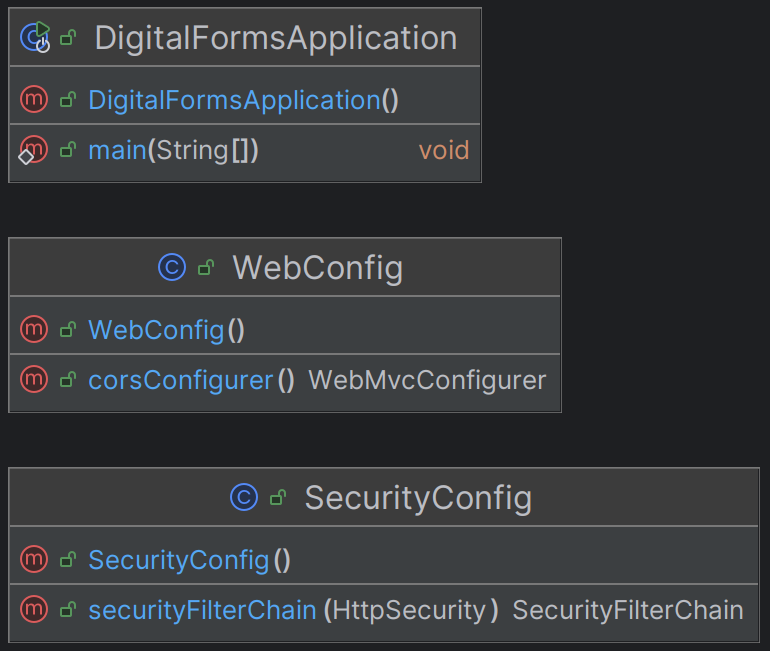
\includegraphics[width=15cm]{images/classDiagrams/Config}
    \caption{Backend Spring Boot Configuration}\label{fig:Backend-Spring-Boot-Configuration}
\end{figure}

\refa{fig:Backend-Spring-Boot-Configuration} zeigt die Konfiguration des Spring Boot Projekts.
Dabei startet "DigitalFormsApplication" das Projekt, "WebConfig" konfiguriert CORS Einstellungen und "SecurityConfig"
Konfiguriert die Zugriffsoptionen auf die Endpunkte.

\begin{figure}[H]
    \centering
    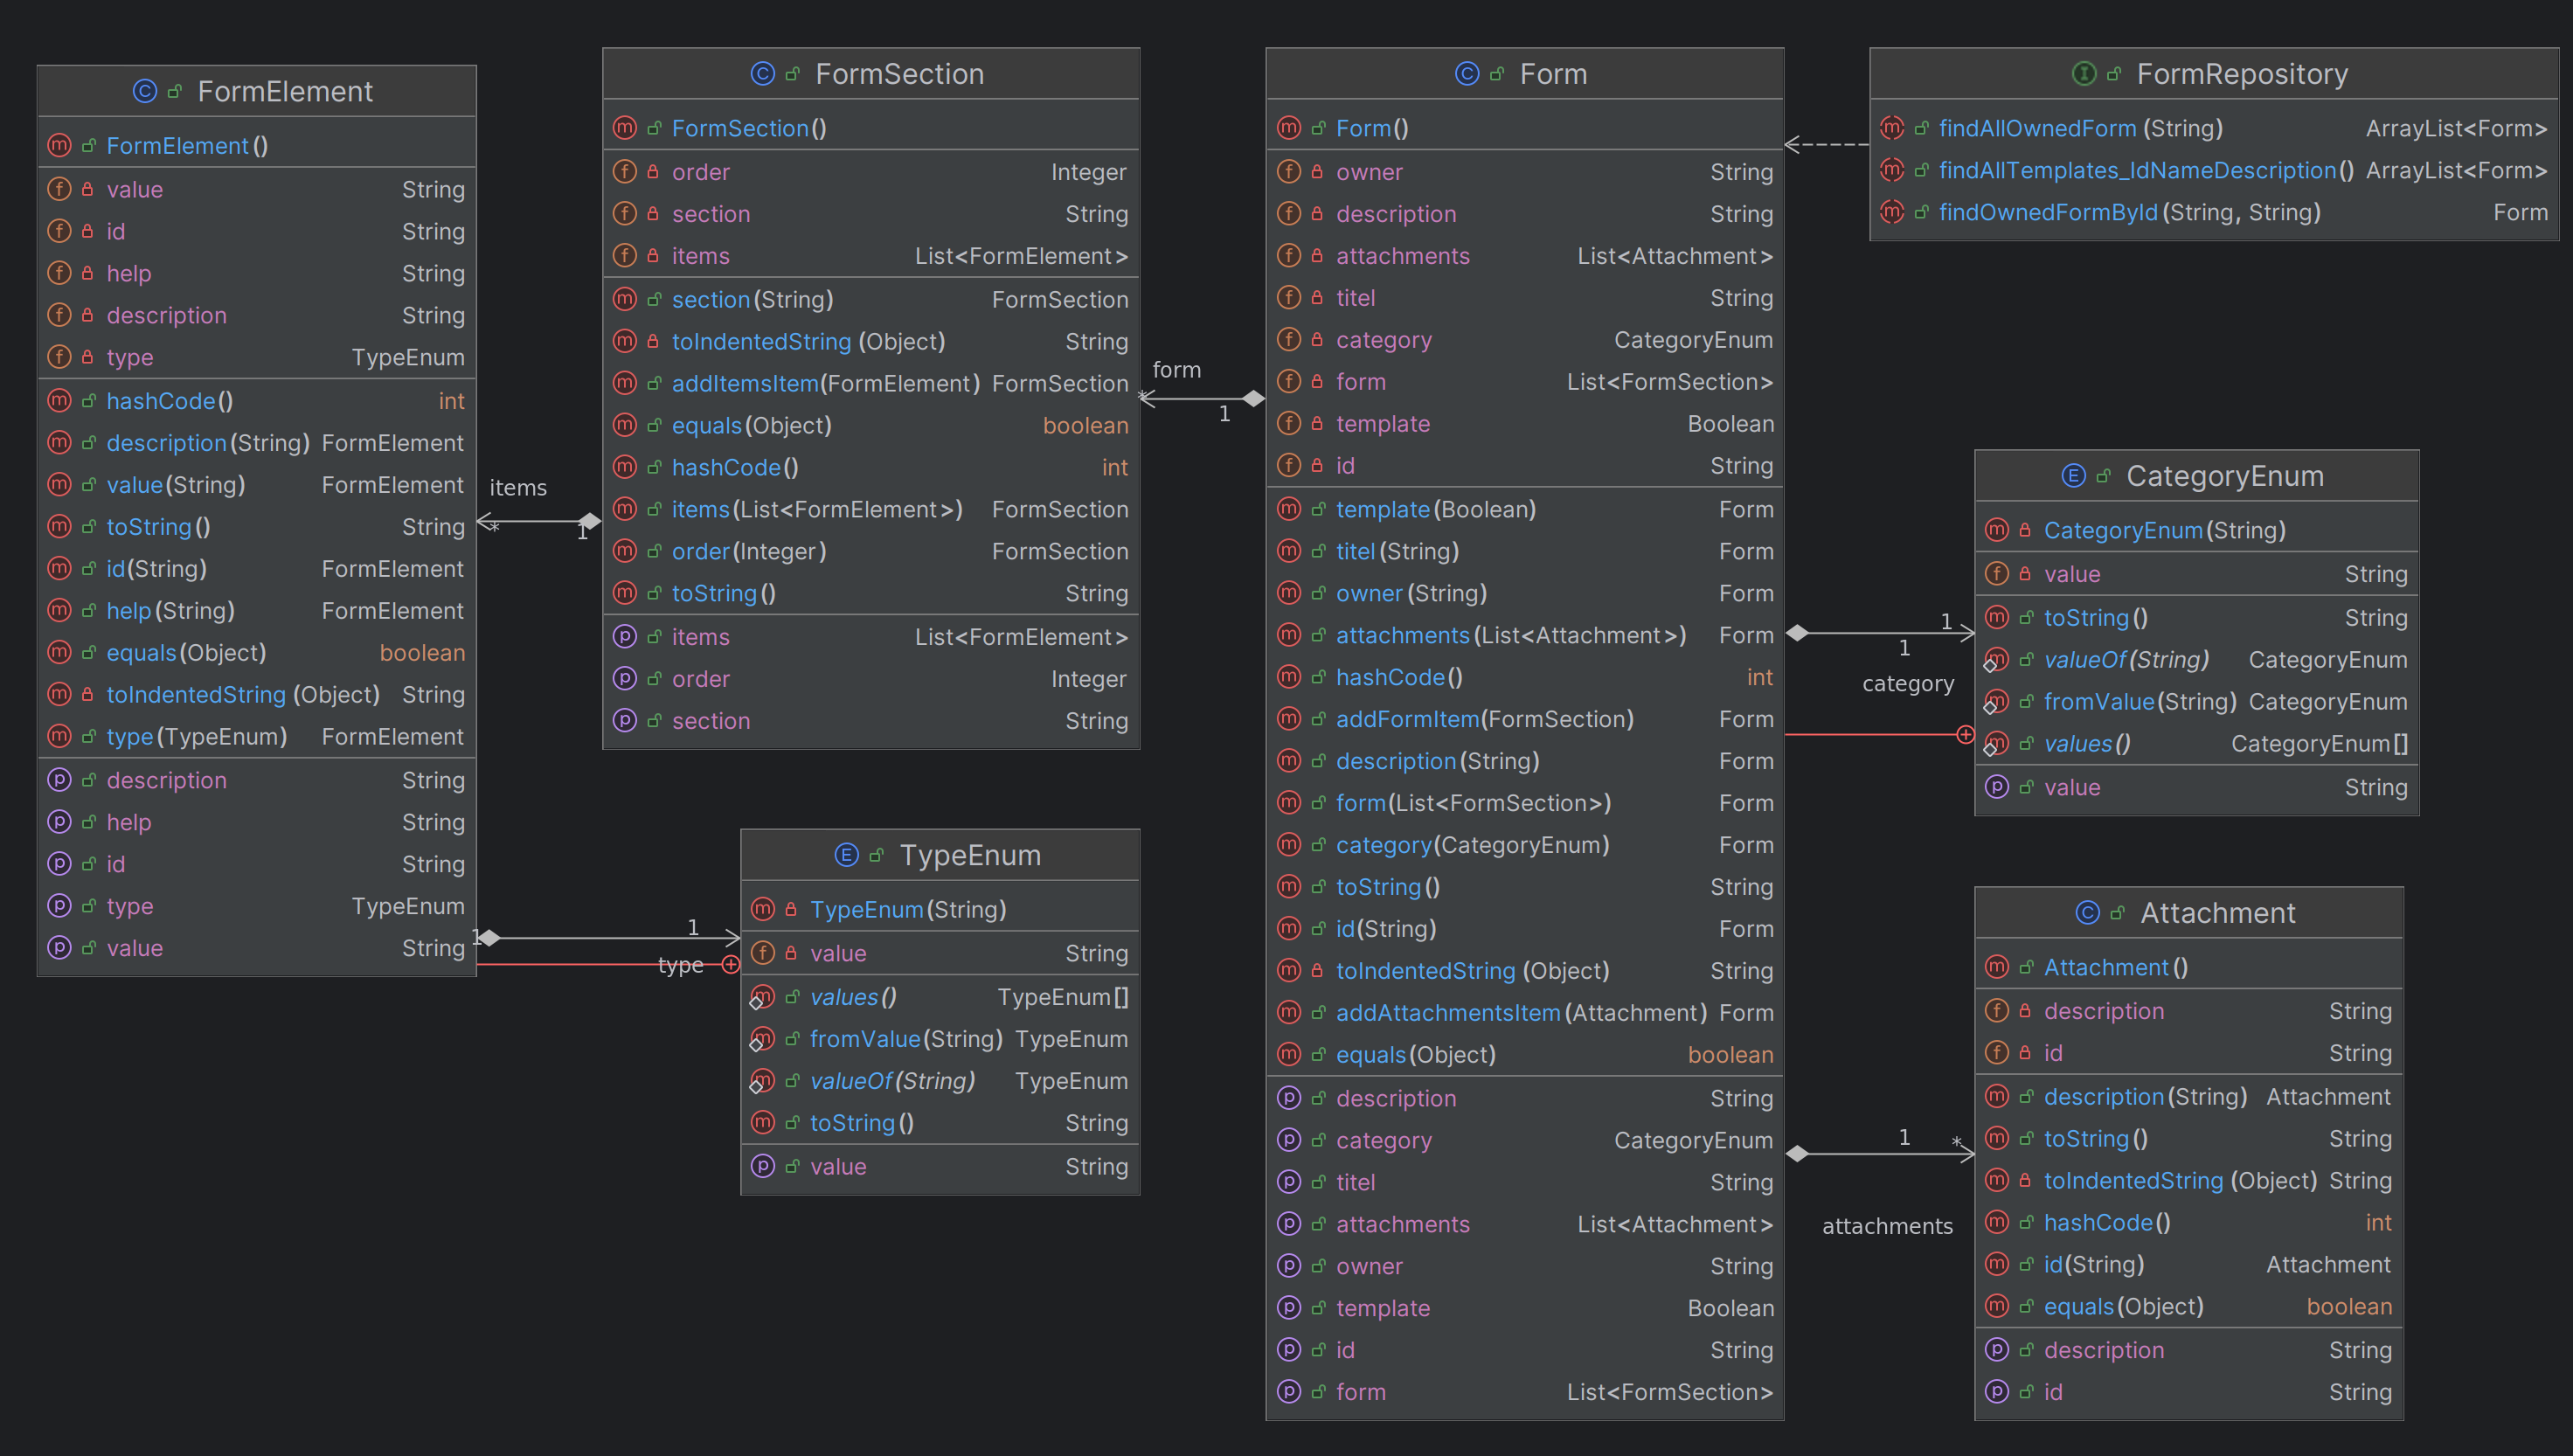
\includegraphics[width=20cm,angle=90,origin=c]{images/classDiagrams/FormRepository}
    \caption{Backend Datenmodell}\label{fig:backendclass-diagram}
\end{figure}

\refa{fig:backendclass-diagram} zeigt den detailarten Aufbau des Datenbankmodells.
Dabei dient "FormRepository" als Schnittstelle für die Datenbank.
Die Objektmodelle werden durch die OpenAPI Spezifikation automatisch generiert.

\begin{figure}[H]
    \centering
    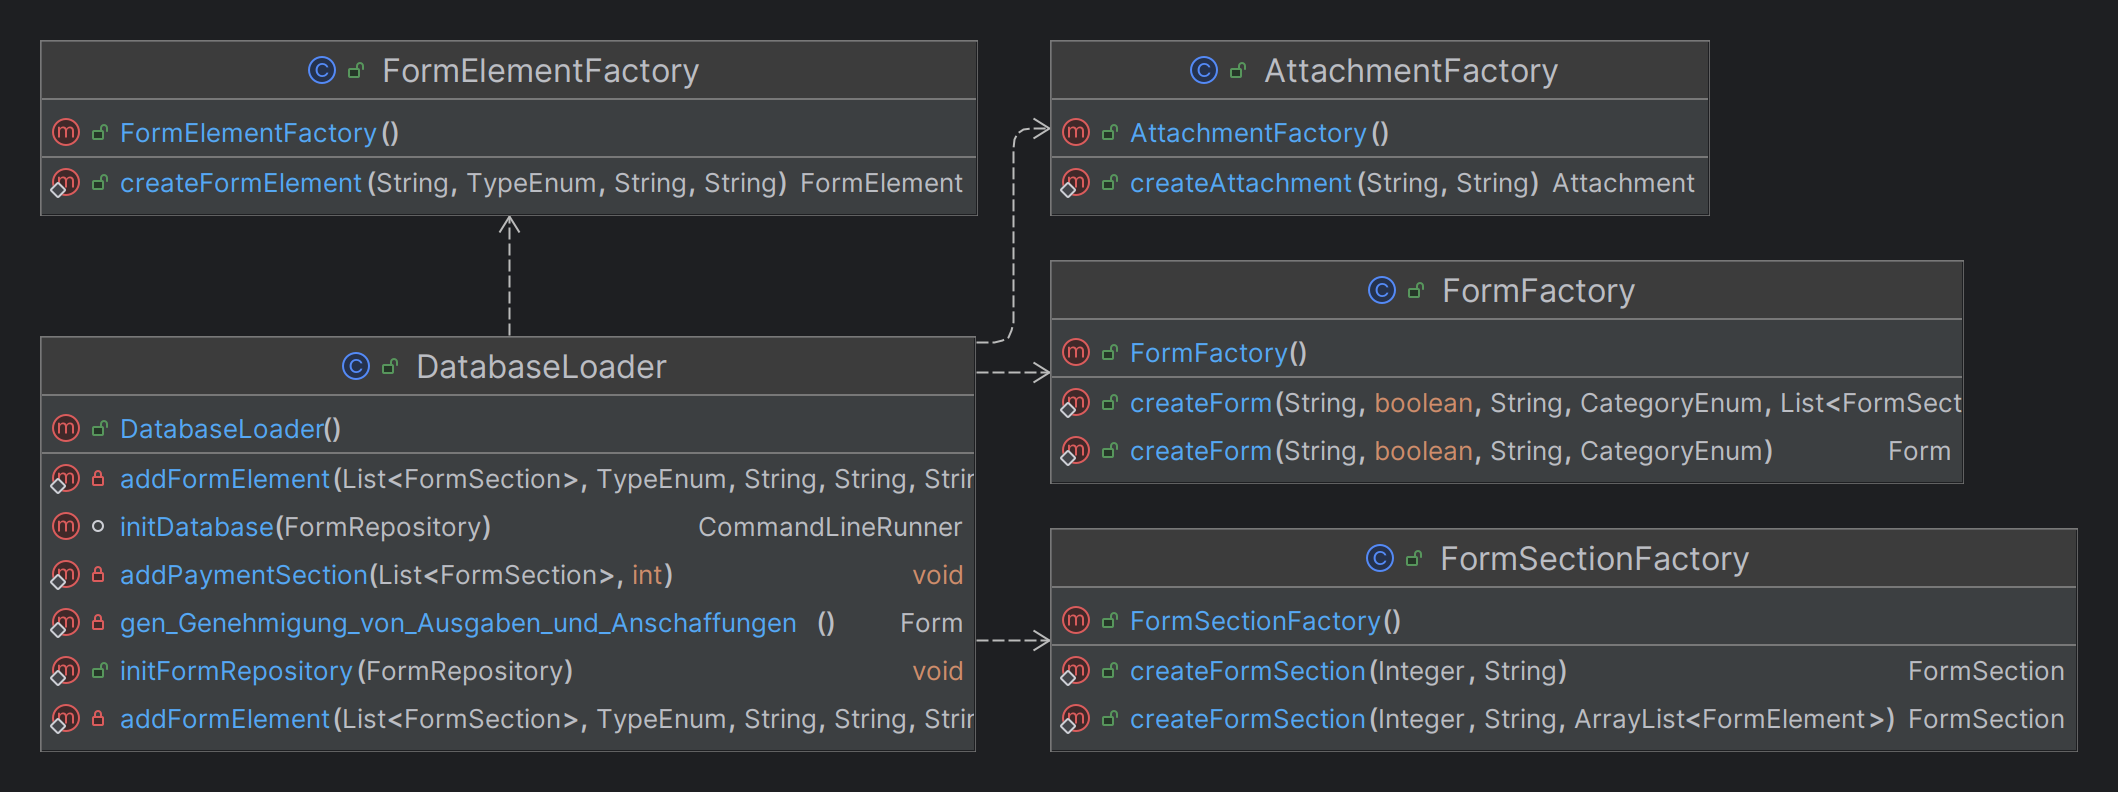
\includegraphics[width=15cm]{images/classDiagrams/DatabaseLoader}
    \caption{Backend Datenbank Init und Factorys}\label{fig:backend-gen-class-diagram}
\end{figure}

Um die Datenbank mit Elementen zu initialisieren, wird der "DatabaseLoader" aus \refa{fig:backend-gen-class-diagram} ausgeführt.
Dieser generiert mithilfe von Factories Elemente für die Datenbank.

\begin{figure}[H]
    \centering
    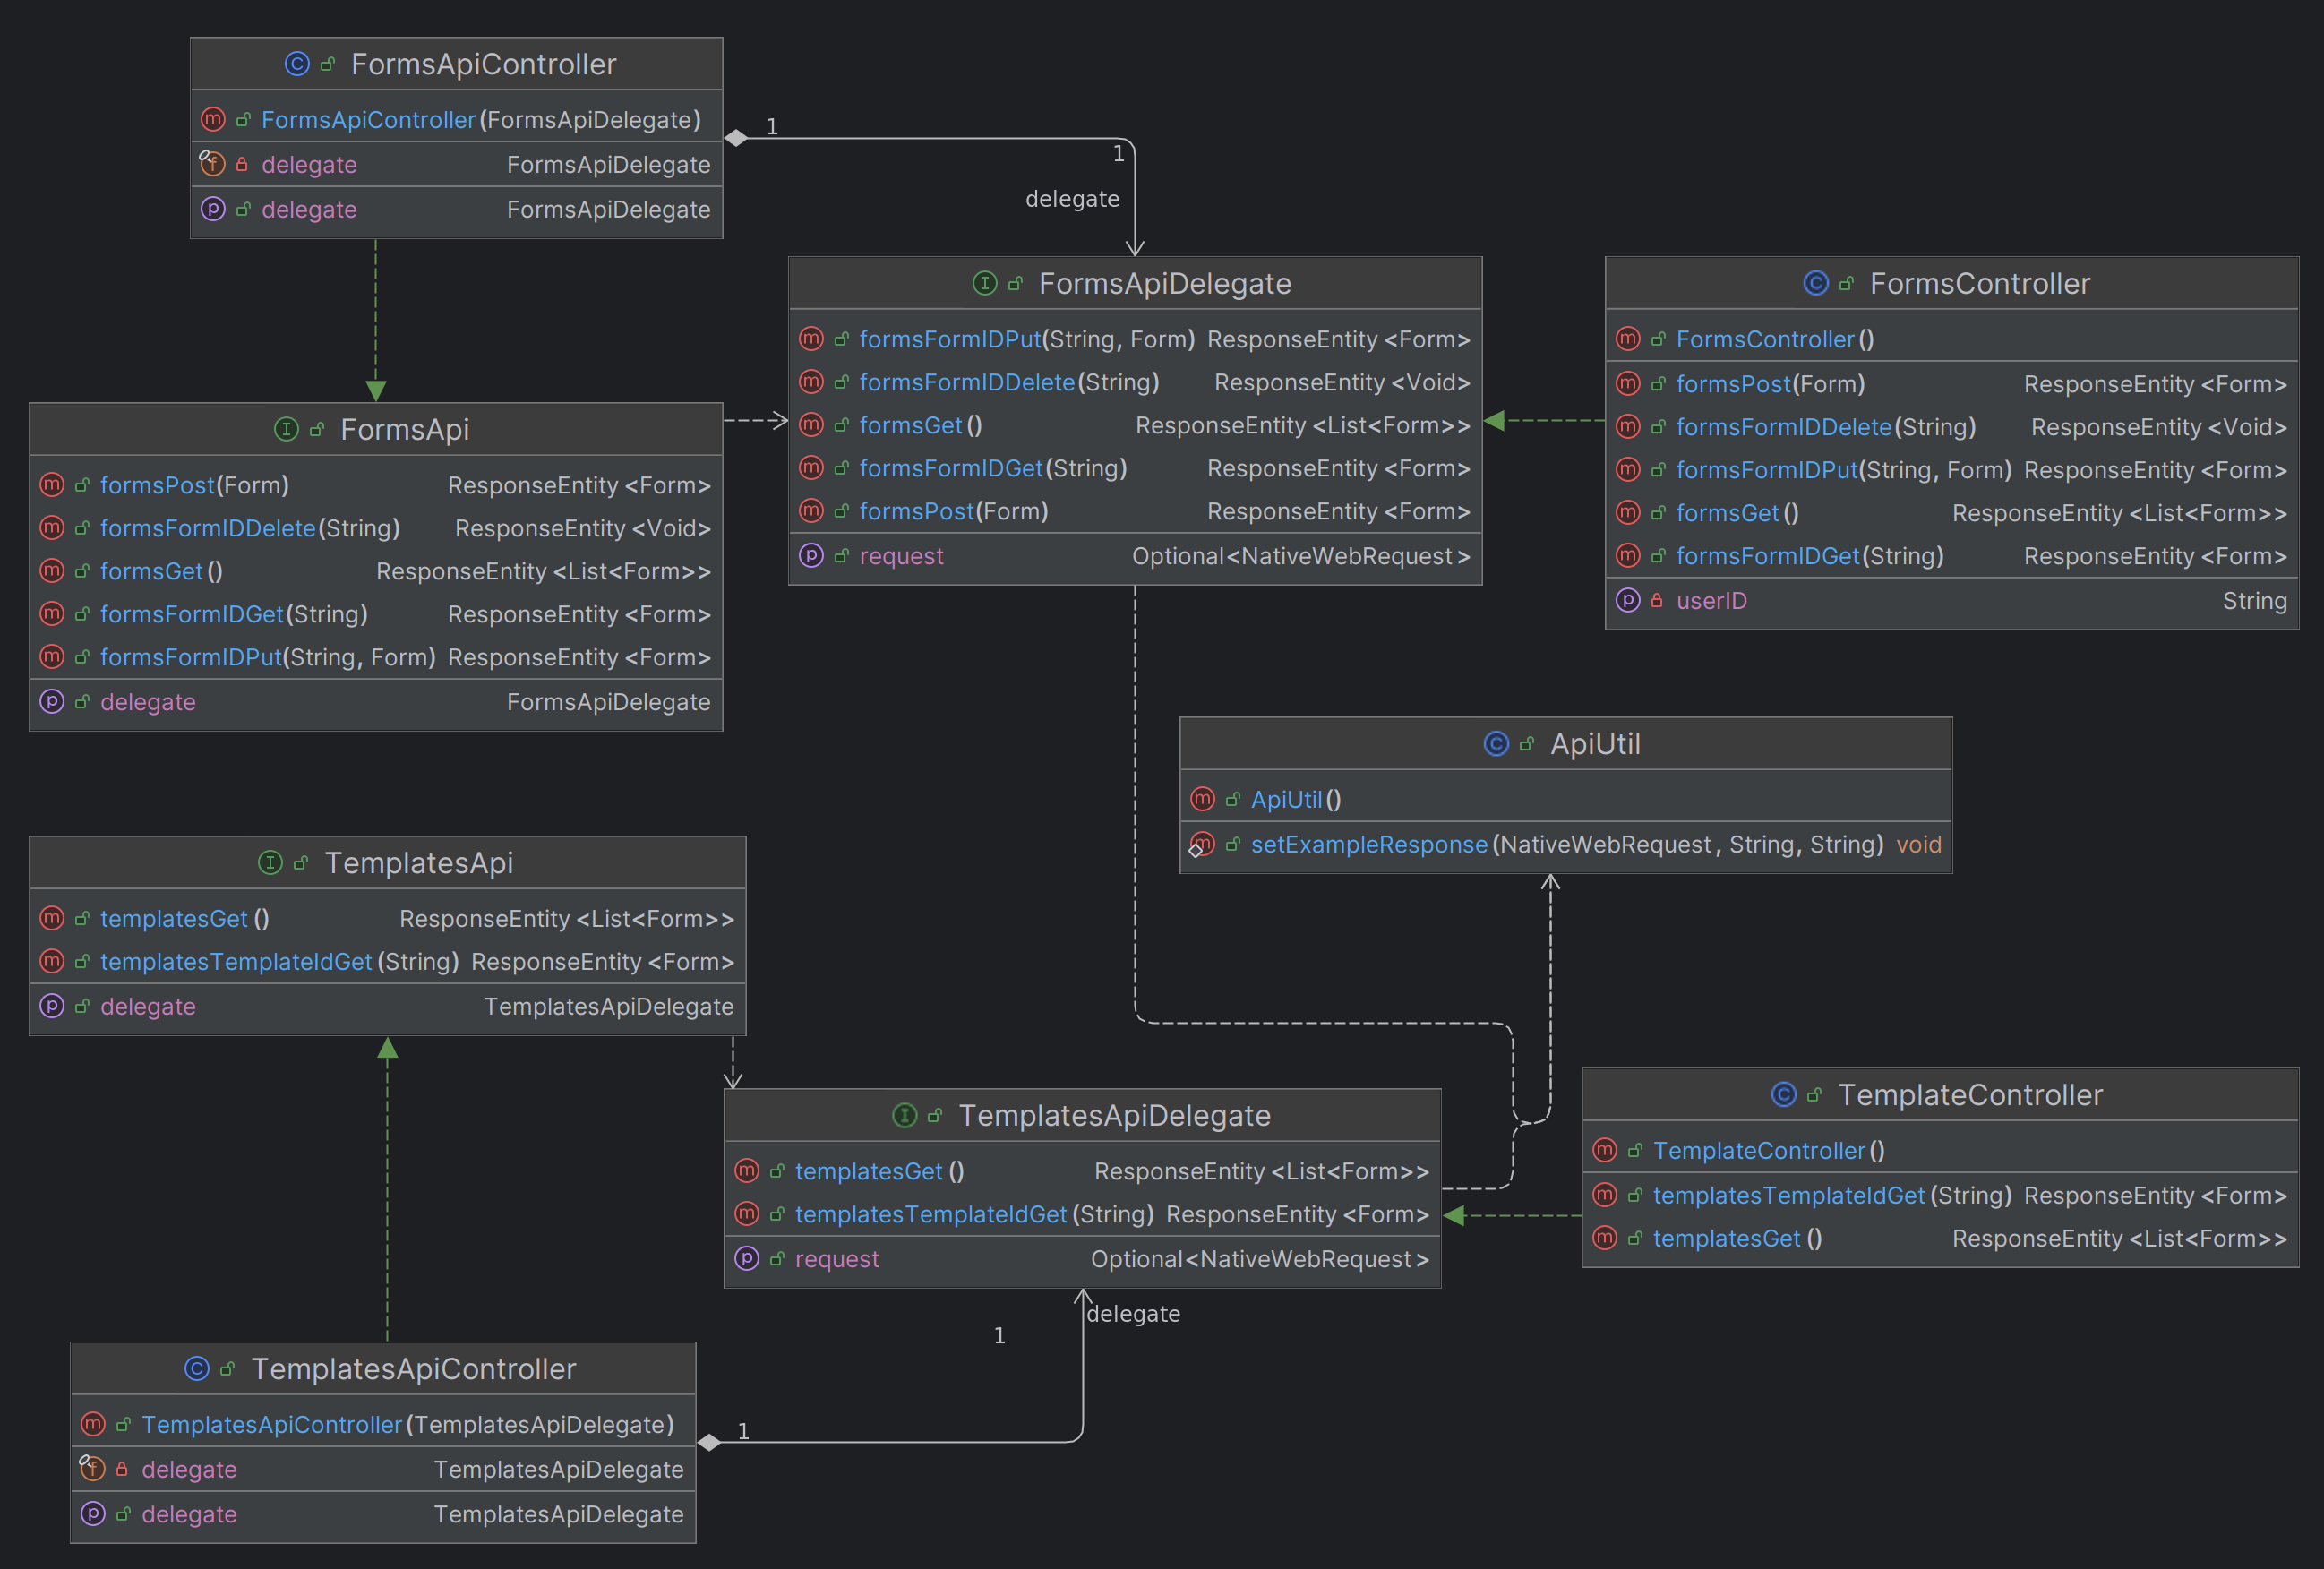
\includegraphics[width=15cm]{images/classDiagrams/Api}
    \caption{Backend API Controller}\label{fig:Backend-API-Controller}
\end{figure}

Die Implementierung der \ac{API} Endpunkte erfolgt in den jeweiligen Controllern.
Diese verwenden generierte Interfaces, wie in \refa{fig:Backend-API-Controller} zu sehen ist.

% \subsection{Frontend}
% Irgendwie Unhappy damit
% Finde Beim Frontend Derzeit nichts Sinfolles

\section{Verhaltensschicht}\label{sec:verhaltensschicht}
Im Folgenden wird das Verhalten der Applikation exemplarisch bei den Usecases Ausfüllen 
eines Antrags, sowie Login beschrieben.

\begin{figure}[H]
    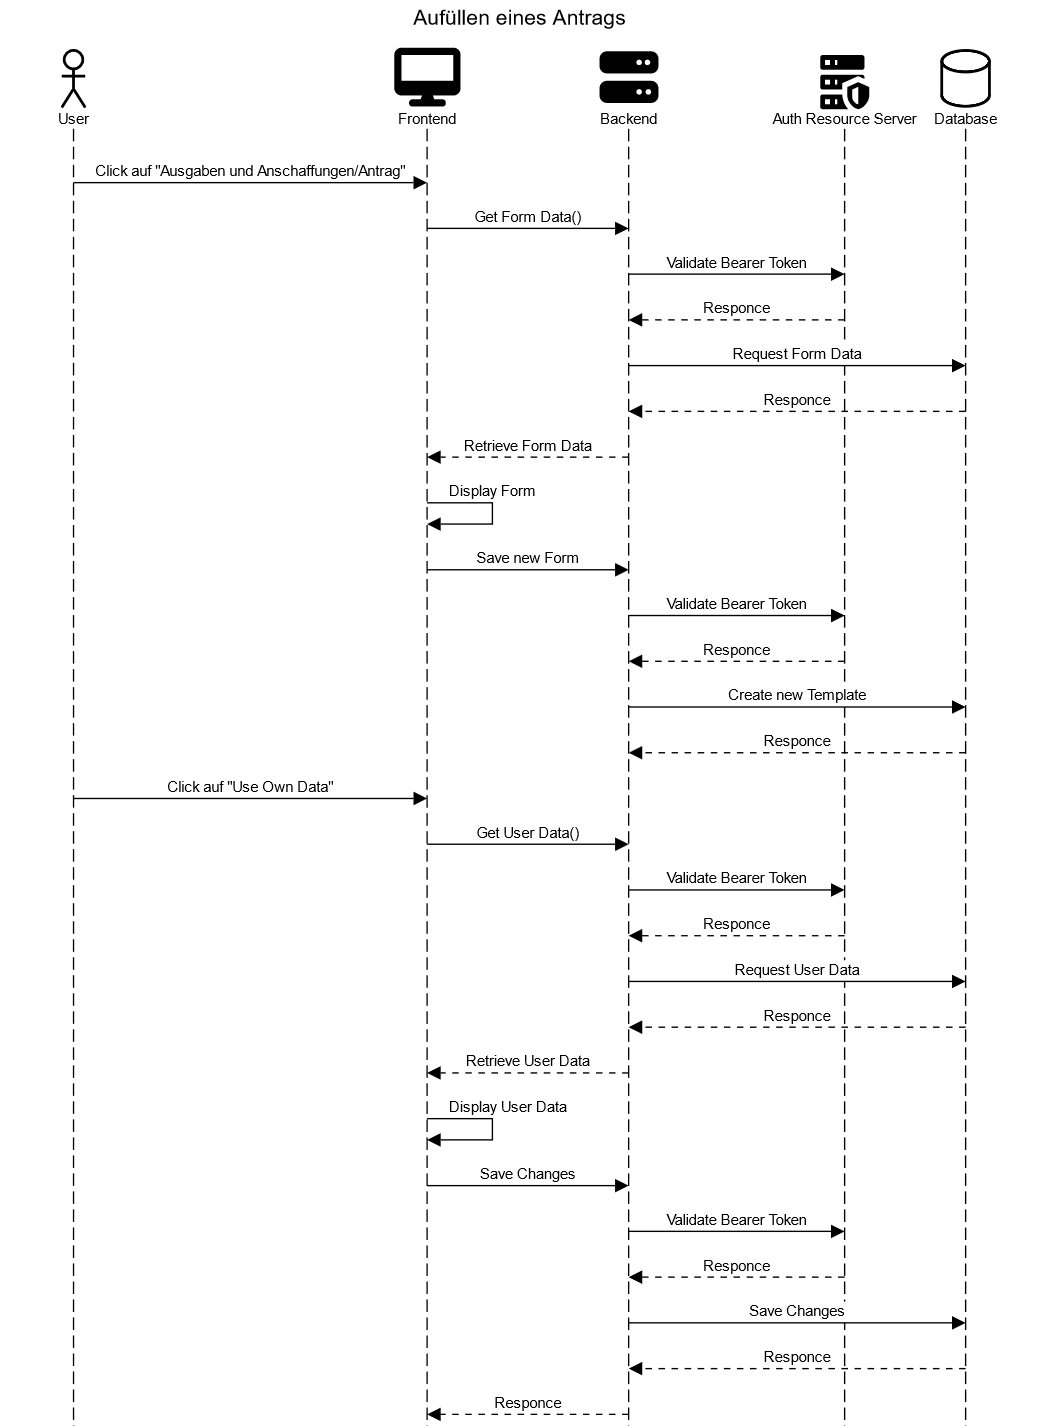
\includegraphics[width=15cm, height=19cm]{Fill_in_Form_Sequence_Diagramm_part_1}
    \caption{Antrag ausfüllen Diagramm Teil 1}\label{fig:Antrag Flow 1}
\end{figure}   
\begin{figure}[H]
    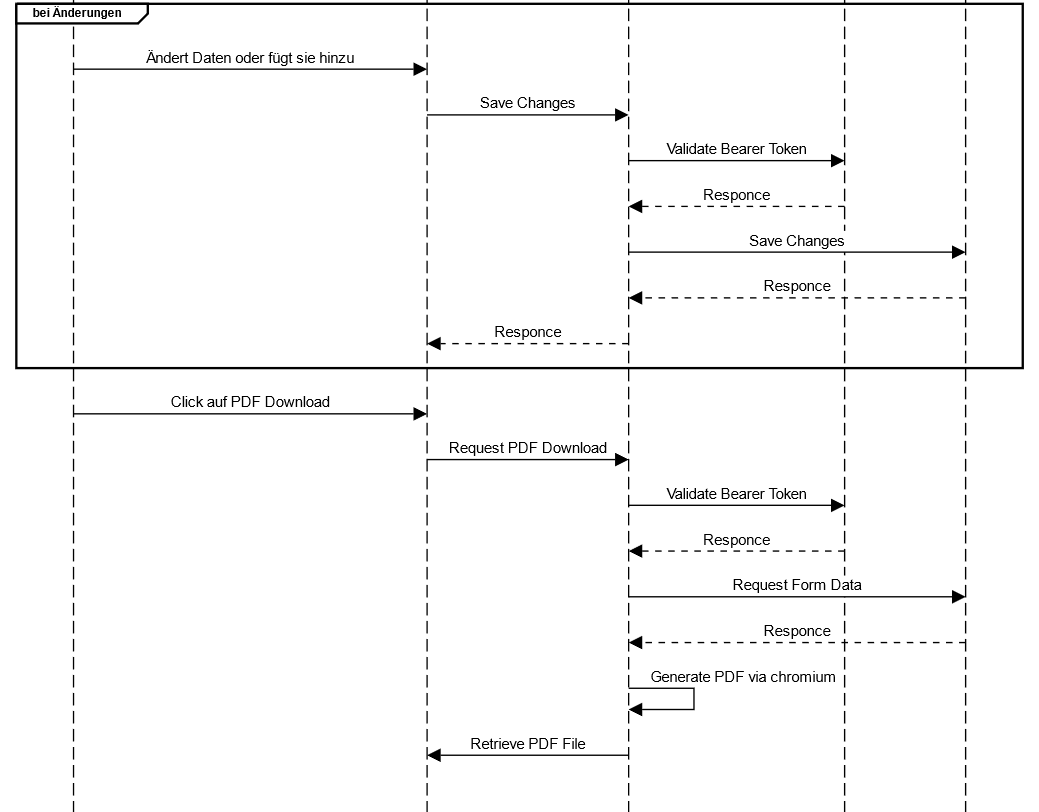
\includegraphics[width=15cm]{Fill_in_Form_Sequence_Diagramm_part_2}
    \caption{Antrag ausfüllen Sequence Diagramm Teil 2}\label{fig:Antrag Flow 2}
\end{figure}
\refa{fig:Antrag Flow 1} und \refa{fig:Antrag Flow 2} zeigen den sequenziellen Ablauf 
und die Interaktionen, die Ablaufen, wenn der Nutzer einen Antrag ausfüllt und dabei 
gegebenenfalls diverse Features wie die Autofill Funktion nutzt.
\begin{figure}[H]
    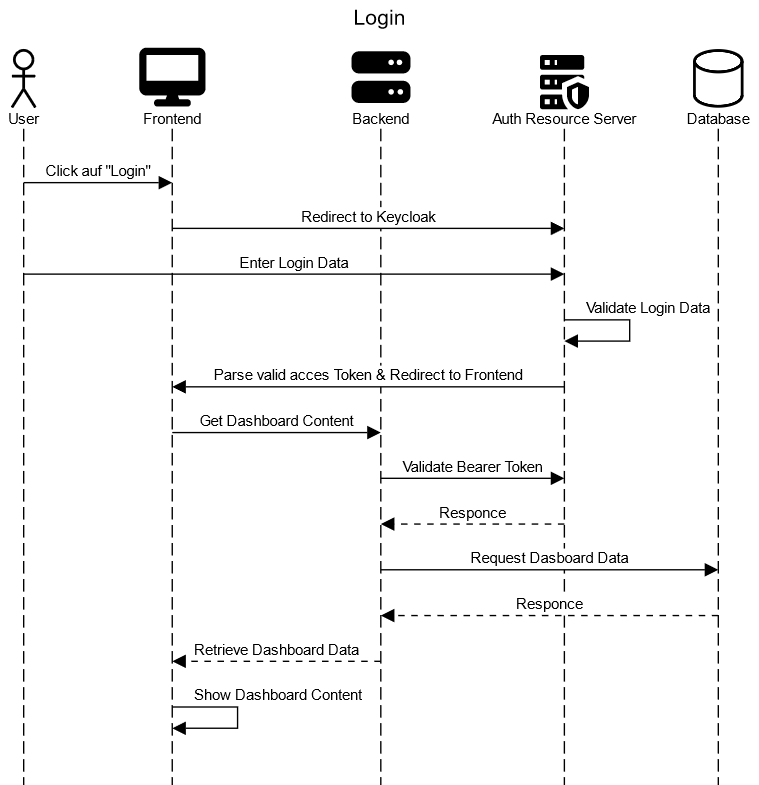
\includegraphics[width=15cm]{Login}
    \caption{Login Sequence Diagramm}\label{fig:Login Flow}
\end{figure}
\refa{fig:Login Flow} zeigt, wie die Applikation eine Authentifizierung des Nutzers und damit 
eine Login-Funktionalität ermöglicht, bzw. wie diese umgesetzt wird.

\section{Verteilungsschicht}\label{sec:verteilungsschicht}
Die Applikation verteilt sich, wie \refa{fig:Netzwerksuebersicht} zeigt, auf drei frei verfügbare Komponenten.
Ein Nutzer kann über die Subdomains "df." für das Frontend, "backend.df." für das Backend und "auth.df."
auf die Komponenten zugreifen.
Das Backend sowie der Authentifizierungsdienst verfügen jeweils zusätzlich über eine lokal verfügbare Datenbank.

\begin{figure}[h]
    \centering
    \includesvg[width=14cm]{./images/GeneralNetwork}
    \caption{Netzwerksübersicht}\label{fig:Netzwerksuebersicht}
\end{figure}

\newpage
\refa{fig:Container-verteilung} zeigt, wie die Anwendung auf einem Server bereitgestellt werden kann.
Dies stellt ebenfalls den Aufbau des verwendeten \ac{CD} Servers dar.
Dieses Projekt stellt die Docker Compose (dargestellt links in \refa{fig:Container-verteilung})
sowie die darin enthaltenen Container zur Verfügung.

Der rechte Teil von \refa{fig:Container-verteilung} empfiehlt die Verwendung von Traefik\footnote{https://traefik.io/traefik/}
als Reverse Proxy.
Die Verwendung eines Reverse Proxy bringt verschiedene Vorteile:
\begin{itemize}
    \item Automatische Redirects von http auf https
    \item Zentrale Absicherung der Dienste mit \ac{SSL}-Verschlüsselung
    \item Routen der Dienste basierend auf deren Subdomain
\end{itemize}

\begin{figure}[h]
    \centering
    \includesvg[width=17cm]{images/ServerSetup}
    \caption{Container verteilung}\label{fig:Container-verteilung}
\end{figure}
   \chapter{Technologien & Frameworks}\label{ch:technologien-&-frameworks}

In diesem Kapitel sind die verwendeten Technologien und Frameworks benannt, erklärt
sowie begründet, weshalb diese verwendet werden.

\section{Angular}\label{sec:angular}

Im Frontend wir Angular für die komponentenbasierte Darstellung verwendet.
Da in Angular die einzelnen Komponenten direkt in solche unterteilt sind,
eignet es sich für den angestrebten modularen Aufbau besonders.

Angular ist eine auf \gls{TypeScript} basierende Entwicklungsplattform, die folgende Funktionalitäten umfasst:
\begin{itemize}
    \item Komponenten basiertes Framework
    \item Eine Vielzahl von stark integrierten Bibliotheken für Routing, Formularmanagement, Client-Server Kommunikation
    \item Entwicklertools zu Entwickel, Testen und Updaten des Codes
\end{itemize}
\cite{about-angular}

Angular ist MIT lizenziert.
Für mehr Details siehe \refk{sec:mit}.

\section{Spring Boot}\label{sec:spring-boot}

Im Backend kommt die bewährte Technologie Spring Boot zu Einsatz.

Spring ermöglicht es Java schneller, leichter und sicherer zu programmieren.
Aufgrund seiner Geschwindigkeit, Einfachheit und Produktivität gilt Spring zum am meisten geschätzten Java-Framework weltweit.
\cite{about-springboot}

Spring Boot ist Apache-2.0 Lizenziert.
Für mehr Details siehe \refk{sec:apache-2.0}.

\section{Keycloak}\label{sec:keycloak}

Keycloak dient, als einfache Möglichkeit, die Applikation abzusichern, ohne selbst Passwörter zu managen.
Zusätzlich wird Benutzer-Föderation, starke Authentifizierung sowie eine Feine Autorisierung bereitgestellt.
\cite{about-keycloak}

Keycloak ist Apache-2.0 Lizenziert.
Für mehr Details siehe \refk{sec:apache-2.0}.

\section{Postgres}\label{sec:postgres}

Postgres dient in diesem Projekt als Datenspeicher für Keycloak.

PostgreSQL ist ein leistungsfähiges, objektrelationales Open-Source-Datenbanksystem.
Es verwendet einen erweiterten SQL Syntax und verfügt über zahlreiche Features,
die es ermöglichen, selbst die komplexesten Daten-Workloads sicher zu speichern und zu skalieren.
\cite{about-postgres}

Postgres steht unter der The PostgreSQL Licence.
Für mehr Details siehe \refk{sec:the-postgresql-licence}.


\section{MongoDB}\label{sec:mongodb}

MongoDB wird zum Speichern der Anträge sowie der Verknüpfung zu den Keycloak Accounts genutzt.
Im Gegensatz zu den klassischen relationalen Datenbanken zählt MongoDB als Dokumenten basierte NoSQL Datenbank.
Dabei werden Information nicht streng auf einzelne Tabellen verteilt, sondern in Form von \ac{JSON} Objekten in Dokumenten abgelegt.

MongoDB steht unter der \acl{SSPL} zur Verfügung.
Für mehr Details siehe \refk{sec:server-side-public-license}.

\section{Docker}\label{sec:docker}

Docker bietet eine unkomplizierte Option, Container zu konfigurieren und zu teilen.
Dabei kann auf Datenbanken mit Basis Images zugegriffen werden, welche bei Bedarf
einfach in einem Dockerfile angepasst werden können.

Docker selbst ist nicht Open Source, jedoch für die meisten kostenlos verfügbar.
Davon ausgeschlossen sind lediglich Firmen mit mehr als 250 Mitarbeitern oder mindestens 10 Millionen Dollar Einkommen.

\section{Docker Compose}\label{sec:docker-compose}

Docker Compose ist eine Erweiterung von Docker.
Diese ermöglicht es direkt mehrere Container in einer Datei zu managen.
Ein weiterer Vorteil stellt die einfache Konfiguration von Docker-Secrets dar, wodurch \ua Passwörter sicher übergeben werden können.

Docker Compose ist Apache-2.0 Lizenziert.
Für mehr Details siehe \refk{sec:apache-2.0}.


   \chapter{APIs}\label{ch:apis}
In diesem Kapitel wird detailierter auf die Verwendung von verschiedenen APIs in unserem Projekt
eingegangen.
   \chapter{Ausblick}\label{ch:ausblick}

Da die Aufgabe unserer Applikation darin besteht, das Ausfüllen von Anträgen so einfach 
und schnell wie möglich zu machen, besteht das größte Potential für Weiterentwicklungen
im Themenbereich der User Experience.

\section{\ac{UI} Design}\label{sec: ui design}
Das momentane \ac{UI} Design beruht auf Kunden und Nutzerfeedback, welches wir in 
Interviews erhalten haben. Zukünftig könnte es von Vorteil sein, solche Interviews 
erneut und mit mehr Probanten durchzuführen, da so eine differenziertere Anaylse
des Feedback und damit das Erstellen eines besseren, auf den Kunden zugeschnittenen \ac{UI} 
Designs ermöglicht werden kann.%ref auf Interviews?

\section{Formular Editor}\label{sec: formular editor}
Auch das Hinzufügen eines Editors für die Erstellung und Manipulation von 
Formular-Templates und der daraus resultierenden PDF wäre eine sinnvolle Erweiterung. Denn 
momentan ist zwar gut dokumentiert, wie neue Anträge in die Applikation eingebunden werden 
können, dies erfordert jedoch das direkte Manipulieren von Dateien in der Applikation 
und ist daher von nicht Fachkundigen Personen nicht durchführbar. Ein visueller Editor, der 
beispielsweise nach einem "Drag and Drop" Prinzip funktionieren könnte, würde diese Lücke 
in der Usability der Applikation schließen, sodass auch IT fremde Nutzer, Anträge 
erstellen, verändern oder löschen können, was die allgemeine User Experience deutlich 
verbessern würde.

\section{Wiederverwenden von Antragsdaten}\label{sec: wiederverwenden von Antragsdaten}
Eine weitere potentielle Verbesserung der User Experience bestünde in der Möglichkeit, 
Daten, welche in einem bestimmten Antrag verwendet wurden, direkt in ein 
Abrechnungsformular zu übernehmen. Dies könnte durch eine neue Entität in der Datenbank, 
oder durch Import einer passenden Datei ermöglicht werden, ähnlich wie es bereits im 
Autofill Feature der Fall ist. Dadurch ließe sich beim Ausfüllen einer Abrechnung deutlich 
mehr Zeit sparen, was eine bessere User Experience zur Folge hätte.%Autofill ref

\section{Maps \ac{API}}\label{sec: maps api}
Um das Ausfüllen von Anträgen wie der Reisekostenerstattung weiter zu vereinfachen, würde 
sich die Integration einer Karten-\ac{API} anbieten. Wenn man also beispielsweise im 
Antrag angeben muss, von wo man startet, wo man hinfährt, und welche Zwischenstopps man 
macht, könnte dies durch einfache Klicks auf einer interaktiven Karte passieren. Zusätzlich 
könnten weitere Daten wie vorraussichtliche Treibstoffkosten, vorraussichtliche Reisedauer 
und andere wichtige Daten auf Basis dieser Funktion errechnet, und direkt in den Antrag 
integriert werden. Auch ein Anhängen der Karte mit visualisierter Route an die generierte
PDF als Beleg der Daten, wäre möglich. So ließe sich das mühsame Eingeben von Adressen 
und die damit einhergehende Fehleranfälligkeit umgehen. Dies würde es den Nutzern 
ermöglichen, den Antrag schneller und einfacher auszufüllen und würde damit die User 
Experience deutlich verbessern.

\section{Verwalten von Accounts}\label{sec: verwalten von Accounts}
Momentan müssen die Nutzeraccounts der Applikkation vollständig von einem fachkundigen 
Administrator verwaltet werden. Dies schließt das Erstellen neuer Accounts, sowie das 
Ändern von Passwörtern und Nutzernamen ein. Es wäre jedoch wünschenswert, wenn jeder 
Nutzer über ein geeignetes \ac{UI} die Möglichkeit hätte, die eigenen Login Daten selbst 
zu verwalten um so zum Einen den Administrator zu entlasten und zum Anderen selbst mehr 
Einfluss auf den eigenen Account zu haben. Dies würde die User Experience deutlich 
verbessern, da zum Ändern der Logindaten bzw. zum Erstellen einnes Accounts keine 
Konsultation des Administrators mehr nötig ist, was den Prozess deutlich vereinfacht und 
beschleunigt.

\section{Login mit anderen Accounts}\label{sec: login mit anderen Accounts}
Da die meisten Nutzer bereits über Accounts in einigen der gängigsten Web Dienste verfügen, 
wäre es für eine gute Usability von Vorteil, wenn man sich nicht nur über den 
applikationseigenen Account bei Keycloak, sondern beispielsweise auch über den Google 
Account anmelden könnte. So könnte man das zeitintensive Erstellen und Verwalten eines 
weiteren Accounts vermeiden. Welche Web Dienste integriert werden könnte auf Basis des in 
16.1 genannte Interviews entschieden werden.
   \chapter{Datenbank}
Da in diesem Projekt eine NoSQL Datenbank verwendet wird, gibt es kein Datenbanklayout im klassischen Sinne.
Regeln für die Strukturierung von Daten wie Normalformen bei Relationalen Datenbanken gibt es bei MongoDB nicht.

Dennoch gibt es einige Punkte die zu beachten sind:
\begin{itemize}
    \item Limit von 16\ac{MB} Pro Dokument
    \item Einbetten ist bei NoSQL Datenbanken zu bevorzugen, jedoch nicht immer passend
    \item Arrays sollten nicht unendlich wachsen können
\end{itemize}

Es folgt die vorläufige Struktur für die verschiedenen Dokumente.

\section{Userdata / Autofill}

\begin{lstlisting}[label={lst:lstlistingusers}]
    // userData Document
    {
      "_id": {"$oid": string},
      "IBAN": string,
      "_class": "de.PSWTM.DigitalForms.model.UserData",
      "adress": string,
      "creditInstitute": string,
      "email": string,
      "firstName": string,
      "name": string,
      "userId": string
    }


\end{lstlisting}

\section{Template PDF}
\begin{lstlisting}[label={lst:lstlistingauto}]
    // templatePDF Document
    {
      "_id": {"$oid": string},
      "_class": "de.PSWTM.DigitalForms.Model.TemplatePDF",
      "formId": string,
      "templatePdf": string
    }

\end{lstlisting}

\section{Template Gruppe}
\begin{lstlisting}[label={lst:templateGroup}]
    // templateGroup Document
    {
      "_id": {"$oid": string},
      "_class": "de.PSWTM.DigitalForms.model.TemplateGroup",
      "antragId": string,
      "description": string,
      "reasons": [string, string],
      "rechnungen": [string, string],
      "titel": string
    }

\end{lstlisting}


\section{Favourite}
\begin{lstlisting}[label={lst:favourite}]
    // favourite Document
    {
      "_id": {"$oid": string},
      "_class": "de.PSWTM.DigitalForms.model.Favourite",
      "formId": string,
      "owner": string
    }

\end{lstlisting}


\section{Form}\label{sec:form}
Das Form-Dokument definiert die Struktur, in welcher Formulare gespeichert werden.
Hierbei werden verschiedene \gls{enum}s verwendet, welche im Folgenden näher beschrieben werden.


'TypeEnum' beschreibt die verschiedenen Feldtypen, welche dargestellt werden sollen.
\begin{lstlisting}[label={lst:TypeEnum}]
    public enum TypeEnum {
        text,
        address,
        iban,
        date,
        money,
        TextMultiLine,
        bool
    }
\end{lstlisting}


'CategoryEnum' ermöglicht die Unterteilung eines Formulars in fest definierte Kategorien
\begin{lstlisting}[label={lst:CategoryEnum}]
    public enum CategoryEnum {
        Antrag,
        Abrechnung
    }
\end{lstlisting}


'RequiredEnum' teilt Anhänge in einen von 3 Typen ein.
Dabei steht die Option zwischen, immer notwendig, eventuell notwendig, je nach bedingung notwendig.
\begin{lstlisting}[label={lst:RequiredEnum}]
    public enum RequiredEnum {
        always,
        user,
        conditional
    }
\end{lstlisting}


Das Form-Dokument selbst ist im Folgenden beschrieben.
Der Boolean "Template" dient hierbei zur Unterscheidung zwischen
Form-Dokumenten, welche beschreiben, wie das Formular dem Nutzer
dargestellt werden soll, sowie Form-Dokumenten, welche Daten enthalten.

Sollte es sich nicht um eine Vorlage zum Ausfüllen handeln, so werden nur die notwendigen Informationen erfasst.
\begin{lstlisting}[label={lst:lstlistingdoc}]
    {
      "_id": {"$oid": string},
      "_class": "de.PSWTM.DigitalForms.model.Form",
      "template": bool,
      "titel": string,
      "category": CategoryEnum,
      "description": string,
      "form": [
        {
          "order": integer,
          "section": string,
          "items": [
            {
              "_id": string,
              "description": string,
              "type": TypeEnum,
              "value": string
            },
            {
              "_id": string,
              "description": string,
              "type": TypeEnum,
              "value": string
            }
          ]
        },
        {
          "order": integer,
          "section": string,
          "items": [
            ...
          ]
        },
        {
          ...
        }
      ],
      "attachments": [
        {
          "_id": string,
          "description": string,
          "required": RequiredEnum,
          "conditionRef": string,
          "conditionRefVal": string,
          "help": string
        }
      ]
    }

\end{lstlisting}
   \newcommand{\trWork}[6]
{
    \multicolumn{1}{|l|}{\textbf{\begin{tabular}[c]{@{}l@{}}#1\end{tabular}}} &
    \multicolumn{1}{l|}{\begin{tabular}[c]{@{}l@{}}#2\end{tabular}} &
    \multicolumn{1}{l|}{#3} &
    \\ \cline{1-3}
    \begin{tabular}[c]{@{}l@{}}#4\end{tabular} &
    \multicolumn{2}{l}{\begin{tabular}[c]{@{}l@{}}#5\end{tabular}} &
    \multirow{\begin{tabular}[c]{@{}l@{}}#6\end{tabular}} \\ \hline
}
\newcommand{\gitIssue}[1]
{
    \href{https://github.com/MaxTrautwein/AStA-Digital-Forms/issues/#1}{Issue #1}
}
\newcommand{\gitPull}[1]
{
    \href{https://github.com/MaxTrautwein/AStA-Digital-Forms/pull/#1}{PR #1}
}
\newcommand{\gitCommit}[2]
{
    \href{https://github.com/MaxTrautwein/AStA-Digital-Forms/pull/#1/commits/#2}{\StrLeft{#2}{10}}
}

\chapter{Aufteilung des Teams}\label{ch:aufteilung-des-teams}
Die Aufteilung der Aufgaben wurde in den Sprint plannings im Einvernehmen des Teams bestimmt.
Im Nachfolgenden sind die erreichten Leistungen sowie die dafür aufgewendet Zeit dokumentiert.
Zu keinem Zeitpunkt war die Arbeit durch Fehlen von Aufgaben blockiert.

\section{Nicht gemessene Zeitaufwände}\label{sec:nicht-gemessene-zeitaufwande}
Das Messen der aufgewendeten Zeit für Tickets war vorgeschrieben und wurde beachtet.
Jedoch fällt nicht jede getätigte Arbeit unter Tickets, welches sich besonders für direkte inhaltliche Arbeiten eignen.

So wurden die Aufgewendeten zeiten für die folgenden Tätlichkeiten nicht erfasst.
\begin{itemize}
    \item Reviews
    \item Meeting Zeit
    \item Unterstützung
    \item Protokoll schreiben
    \item Protokoll/ Meetings vorbereiten
    \item Sprint Plannings
\end{itemize}
Da diese Zeiten in keinster Weise insignifikant waren, wäre es sinnvoll gewesen, auch diese genauer zu dokumentieren.

\section{Ganzes Team}
Einige der Tätlichkeiten wurden vom ganzen Team ausgeübt.
Nicht alle dieser wurden Zeitlich genau dokumentiert.

\subsection{Doku & Planung - Funktionsumfang & Aufwandsschätzung}
8h
https://github.com/MaxTrautwein/AStA-Digital-Forms/issues/7
für die Planung Selbst

\subsection{Spike - Backend Technologie wahl }
15min
https://github.com/MaxTrautwein/AStA-Digital-Forms/issues/11

\section{Max Trautwein}\label{sec:max-trautwein}

total: 1h 5min + 30min + 1h 15min + 6h + 5h 30min + 1h + 3h + 5h 30 + 30min + 5h 30min + 1h + 45min + 4h 15min + 1h
+ 8h 30min + 6h 30min + 30min + 10h 45min + 2h 30min + 6h + 31h 22min + 3h 15min + 45min + 12h 10 min + 5h 30min + 6h 35min
+ 15min + 20min + 45min

=> 132h 32min

% \trWork{Title}{-}{Time}{-}{\gitIssue{1} \\ \gitPull{2}}{-}
    \begin{longtable}{|llll|}
        \hline
        \rowcolor[HTML]{9B9B9B}
        \multicolumn{1}{|l|}{\cellcolor[HTML]{9B9B9B}} &
        \multicolumn{2}{l|}{\cellcolor[HTML]{9B9B9B}\textbf{Links}} &
        \cellcolor[HTML]{9B9B9B} \\ \cline{2-3}
        \rowcolor[HTML]{9B9B9B}
        \multicolumn{1}{|l|}{\multirow{\cellcolor[HTML]{9B9B9B}\textbf{Titel \& Description}}} &
        \multicolumn{1}{l|}{\cellcolor[HTML]{9B9B9B}\textbf{Requierment}} &
        \multicolumn{1}{l|}{\cellcolor[HTML]{9B9B9B}\textbf{Aufwand}} &
        \multirow{\cellcolor[HTML]{9B9B9B}Sprint / Date} \\ \hline
        \endhead
        \trWork{Repo Init}{Init}{1h 5min}{Inizialisirung des GitHub Repositorys\\mit der Dokumentation}{\gitIssue{1} \\ \gitPull{2}}{-}

        \trWork{Documentation prep Milestone 1}{Doku}{30min}{Erstellung aller Chapters\\Verlinkung in der main.tex}{\gitIssue{3} \\ \gitPull{4}}{-}
        \trWork{Randbedingungen}{Doku}{1h 15min}{Dokumentation der Randbedingunen}{\gitIssue{6} \\ \gitPull{15}}{-}
        \trWork{Planung - Funktionsumfang \\ \& Aufwandsschätzung}{Doku}{6h}{Dokumentation des Funktionsumfangs\\sowie der Aufwandsschätzung}{\gitIssue{7} \\ \gitPull{16}}{-}
        \trWork{Planung - Architektur}{Doku}{5h 30min}{Architektur Design und Dokumentation\\Erstellung von Visualisirung}{\gitIssue{9} \\ \gitPull{12}}{-}
        \trWork{Allgemeine Anpassungen Doku}{Doku}{1h}{Verschidene Anpassungen vor der ersten Abgabe}{\gitIssue{18} \\ \gitPull{21}}{-}
        \trWork{Präsentation Vorbereiten}{Doku}{3h}{Vorbereitung auf die erste Präsentation}{\gitIssue{22}}{-}
        \trWork{Docker Compose Setup}{NF-\ref{subsec:dockerized}\\init}{5h 30 min}
        {Inizalisirung des Frontends und Backends\\Erstellungs des Docker-Compose\\Testen auf verschidenen Systemen\\Doku in Redme}{\gitIssue{24} \\ \gitPull{31}}{-}
        \trWork{Durchführung Interviews}{NF-\ref{subsec:bedienung/layout}}{30min}{Durchführung der Interviews}{\gitIssue{27}}{-}
        \trWork{Technologien \& Frameworks}{Doku}{5h 30min}
        {Dokumentation der Verwendeten\\Technologien sowie Frameworks\\Dokumentation der Lizenzen}{\gitIssue{28} \\ \gitPull{41}}{-}
        \trWork{Datenbankmodell}{Doku}{1h}{Dokumentation eines\\vorläufigen Datenbankmodells}{\gitIssue{29} \\ \gitPull{40}}{-}
        % Alternativ könnte das auch auf Docker linken
        \trWork{Setup Keycloak Deployment}{NF-\ref{subsec:technologie}}{45min}{Configuration von Keycloak}{\gitIssue{32}}{-}

        \trWork{Setup CI/CD}{Extra}{4h 15min}{Einrichtung Server\\Erstellung Deploy Patch & Script\\Configuration Workflow\\Initziale Dokumentation davon}{\gitIssue{33} \\ \gitPull{51} \\ \gitPull{53}}{-}
        \trWork{Datenbank Verbindung Backend}{Support}{1h}{Bereitstellung eines Beispiels}{\gitIssue{49}}{-}
        \trWork{Config Konzept}{F-\ref{subsec:dynamischer-formular-aufbau}}{8h 30min}
        {OpenAPI Specifikation\\Erstes realles Datetenbanklayout\\Füllen der Datenbank mit ersten Formularen\\in der entwikelten Struktur\\Dokumentation dessen}{\gitIssue{50} \\ \gitPull{60}}{-}
        \trWork{Barebones Form}{F-\ref{subsec:dynamischer-formular-aufbau}}{6h 30min}
        {Erstellung eines Systems zur dynamischen\\anzeige eines Formulars bestehend aus\\Dynamischen Inhalt}{\gitIssue{66} \\ \gitPull{72}}{-}
        \trWork{\ac{CORS}\\ Setting in Backend \\with OpenAPI}{-}{30min}{Behebung von problemen mit \ac{CORS}}{\gitIssue{67} \\ \gitPull{69}}{-}
        \trWork{Feature Speichern \\(+ Laden im Backend \& API)}{F-\ref{subsec:persistente-antragsbearbeitung}}{10h 45min}
        {Erweiterung der OpenAPI Spezifikation\\Erstellung von Endpunkten zum\\Speichern und Laden\\Erweiterung Frontend zum Speichern}{\gitIssue{75} \\ \gitPull{79}}{-}
        \trWork{Feature Laden Frontend}{F-\ref{subsec:persistente-antragsbearbeitung}}{2h 30min}
        {Frontend Support zum Laden\\bearbeiteter Formulare}{\gitIssue{76} \\ \gitPull{84}}{-}
        \trWork{Architekturschichten Update}{Doku}{6h}
        {Strukturschicht (Class Diagrams)\\Verteilungsschicht (Netzwerk & HW Verteilung)\\Updated Datenbankmodell\\Seperate Appendix File}{\gitIssue{78} \\ \gitPull{85}}{-}
        \trWork{\ac{PDF}}{F-\ref{subsec:pdf-generator}}{31h 22min}
        {Wahl der Generator Technologie\\Form-Template \ac{PDF} Template verlinkung\\OpenAPI Download Endpoint\\Template Logic\\Erstellung der Templates}{\gitIssue{88} \\ \gitPull{100}}{-}
        \trWork{Code Cleanup}{-}{3h 15min}
        {Vorberitung auf Code Review\\Entfernen von Obsoleten Code\\Entfernen unötiger Imports\\Auto Delete leerer Forms}{\gitIssue{89} \\ \gitPull{97}}{-}
        \trWork{Move Done / In Progesss Anträge}{NF-\ref{subsec:bedienung/layout}\\F-\ref{subsec:persistente-antragsbearbeitung}\\F-\ref{subsec:filtermoglichkeiten}}{45min}
        {in Progress / Abgeschlossene Antäge\\auf seperater Seite\\Such Funktion\\Reactive Darstellung}{\gitIssue{105} \\ \gitPull{113}}{-}
        \trWork{Anhangs System}{F-\ref{subsec:anhangs-lieferschein}\\F-\ref{subsec:anhang-system}}{12h 10min}
        {Anhangs Checkliste\\System für Anhangs Typen\\System für Wertabhänige Anhänge\\Tests\\Frontend Seite Überblick\\Verbessern Form Controls}{\gitIssue{107} \\ \gitPull{112}}{-}
        \trWork{Verbessung - Antrags \\ Abrechnungs Linking System}{F-\ref{subsec:antrags-kategorien}\\F-\ref{subsec:auswahls-helfer}\\F-\ref{subsec:filtermoglichkeiten}}{5h 30min}
        {Gruppirung von Antrag zu\\ein oder mehr Abrechnungen\\System zur wahl zwichen\\verschidenen Abrechnungen\\Such funktion\\Reactive Darstellung\\Reactive Favoriten\\Fixed bug requiering reload}{\gitIssue{108} \\ \gitPull{110}}{-}
        \trWork{Setup Installations- und \\Administrationshandbuch}{Doku}{6h 35min}
        {Deployment ‐ Setup Server\\Deployment ‐ Auth Keycloak Config\\Deployment ‐ Domain & Hosting\\
        FAQ Common Issues\\Formular Konfiguration\\PDF Export\\PDF Template Sonderfälle\\Doku, Implementation und Beispiele}{\gitIssue{39} \\ \gitPull{124}}{-}
        \trWork{Setup Aufteilungs Doku}{Doku}{In Progress}
        {Dokumentation der geleisteten Arbeit}{\gitIssue{38}}{-}
        \trWork{added cite for Lizenzen}{Doku}{-}{Quelle für Lizenz infos}{\gitPull{47}}{-}
        \trWork{Fixed issues with DB use in deployment}{-}{-}
        {Einlesen von DB Verbindungs Daten\\über Docker Secrets\\Aktualisierung Compose \\\& Deploy Patch}{\gitPull{56}}{-}
        \trWork{Improved build time on slower \\Internet connections}{-}{15min}{Not Merged wegen wechsel auf Maven\\Caching von dependencies}{\gitPull{58}}{-}
        \trWork{Issue48 login fixes ihope}{-}{20min}{Behebt fehler in \gitPull{55}}{\gitPull{61}}{-}
        \trWork{fixed issues with compile}{-}{-}{Behebt fehler beim Compiele\\füght vergessene dependency hinzu}{\gitPull{62}}{-}
        \trWork{fixed incorrect allowed domain}{-}{-}{Behebt Fehler mit fealscher Domain}{\gitPull{81}}{-}
        \trWork{Added Embedded MongoDB to \\allow tests to run in compose build}{-}{45min}{Ermöglicht Ausführung von Tests}{\gitPull{82}}{-}
        \trWork{fix for mistakes}{-}{-}{Behebt fehler in \gitPull{79}\\Typo und Security}{\gitPull{83}}{-}
        \trWork{Doku3 Final}{Doku}{-}{Behebt fehler in der Docku\\Vor abgabe}{\gitPull{95}}{-}
        \trWork{Async Update}{-}{-}{Not Merged\\Zu Späterem Zeitpukt besser Implementiert}{\gitPull{104}}{-}
    \end{longtable}


\section{Ayhan Yasar}\label{sec:ayhan-yasar}

Total: 2h + 4h + 4h + 1h + 30min + 20h 30min + 14h 30min + 2h + 21h 5min + 1h + 4h + 10min
=> 74h 45min

% \trWork{Title}{-}{Time}{-}{\gitIssue{1} \\ \gitPull{2}}{-}
\begin{longtable}{|llll|}
    \hline
    \rowcolor[HTML]{9B9B9B}
    \multicolumn{1}{|l|}{\cellcolor[HTML]{9B9B9B}} &
    \multicolumn{2}{l|}{\cellcolor[HTML]{9B9B9B}\textbf{Links}} &
    \cellcolor[HTML]{9B9B9B} \\ \cline{2-3}
    \rowcolor[HTML]{9B9B9B}
    \multicolumn{1}{|l|}{\multirow{\cellcolor[HTML]{9B9B9B}\textbf{Titel \& Description}}} &
    \multicolumn{1}{l|}{\cellcolor[HTML]{9B9B9B}\textbf{Requierment}} &
    \multicolumn{1}{l|}{\cellcolor[HTML]{9B9B9B}\textbf{Aufwand}} &
    \multirow{\cellcolor[HTML]{9B9B9B}Sprint / Date} \\ \hline
    \endhead

    \trWork{Planung - Funktionsumfang\\ \& Aufwandsschätzung}{Doku}{2h}{Rechtsschreibkorrektur}{\gitIssue{7}}{-}
    \trWork{Projektmanagement}{Doku}{4h}{Methode, Lizenz, Github Flow\\ und Definition of Done}{\gitIssue{8} \\ \gitPull{13}}{-}
    \trWork{Präsentation Vorbereiten}{Doku}{4h}{Vorbereitung auf die erste Präsentation}{\gitIssue{22}}{-}
    \trWork{Interviews Vorbereiten}{NF-\ref{subsec:bedienung/layout}}{1h}{Erstellen der Fragen}{\gitIssue{26}}{-}
    \trWork{Auswertung Interviews}{NF-\ref{subsec:bedienung/layout}}{30min}{Auswertung der Interview Ergebnisse}{\gitIssue{27}}{-}
    \trWork{Login Implementiren}{F-\ref{subsec:login}}{20h 30min}
    {Login Funktion Frontend\\\ac{JWT} Validirung im Backend}{\gitIssue{48} \\ \gitPull{55}}{-}
    \trWork{Integrate login into Landing page}{NF-\ref{subsec:bedienung/layout}}{14h 30min}
    {Login Seite im Frontend}{\gitIssue{63} \\ \gitPull{73}}{-}
    \trWork{Update Color scheme For Landing page}{NF-\ref{subsec:bedienung/layout}}{2h}{Akktualisirung der Fraben}{\gitIssue{68} \\ \gitPull{86}}{-}
    \trWork{Editor Ausbauen}{-}{21h 5min}
    {Neue Felder für den Editor\\Im Frontend:\\Adresse, Bool, Datum, IBAN,\\Geld, Multiline Text\\Styling Dieser}{\gitIssue{77} \\ \gitPull{103}}{-}
    \trWork{login page}{NF-\ref{subsec:bedienung/layout}}{1h}{Akktualisirung \\Größe und Stiel}{\gitIssue{118}}{-}
    \trWork{Logout Butten}{NF-\ref{subsec:bedienung/layout}}{4h}{Logout Option\\Keine Nav Bar Interaktion ohne Login}{\gitIssue{106}}{-}
    \trWork{Einfuehrung und Ziele Text}{Doku}{10min}{on master via \gitPull{21}}{\gitPull{20}}{-}

\end{longtable}

\section{Tobias Bührle}\label{sec:tobias-buhrle}

total: 2h 30min + 30min + 7h + 3h + 2h 15min + 5h 10min + 30min + 15min + 5h 45min + 5h 10min + 7h 10min
+ 2h 35min + 1h 40min + 30min + 6h 20min + 13h 40min + 12h 10min + 40 min + 1h 25min + 45min + 30min + 55min
+ 2h 25min
=> 82h 50min

% \trWork{Title}{-}{Time}{-}{\gitIssue{1} \\ \gitPull{2}}{-}
\begin{longtable}{|llll|}
    \hline
    \rowcolor[HTML]{9B9B9B}
    \multicolumn{1}{|l|}{\cellcolor[HTML]{9B9B9B}} &
    \multicolumn{2}{l|}{\cellcolor[HTML]{9B9B9B}\textbf{Links}} &
    \cellcolor[HTML]{9B9B9B} \\ \cline{2-3}
    \rowcolor[HTML]{9B9B9B}
    \multicolumn{1}{|l|}{\multirow{\cellcolor[HTML]{9B9B9B}\textbf{Titel \& Description}}} &
    \multicolumn{1}{l|}{\cellcolor[HTML]{9B9B9B}\textbf{Requierment}} &
    \multicolumn{1}{l|}{\cellcolor[HTML]{9B9B9B}\textbf{Aufwand}} &
    \multirow{\cellcolor[HTML]{9B9B9B}Sprint / Date} \\ \hline
    \endhead

    \trWork{Doku - Einführung und Ziele}{Doku}{2h 30min}{-}{\gitIssue{5} \\ \gitPull{17}}{-}
    \trWork{Doku \& Planung - Funktionsumfang\\ \& Aufwandsschätzung}{Doku}{30 min}{-}
    {\gitCommit{16}{33a47b39aae996437d0e8a44f02ad4f1d116f8fb} \\ \gitCommit{16}{bd358a830650a1d39ce75798687fc2956a6a299c}}{-}
    \trWork{Doku \& Erstellen - UI Design}{Doku}{7h}{-}{\gitIssue{10} \\ \gitPull{14}}{-}
    \trWork{Präsentation Vorbereiten}{Doku}{3h}{-}{\gitIssue{22}}{-}
    \trWork{User Stories}{Doku}{2h 15min}{-}{\gitIssue{23} \\ \gitPull{30}}{-}
    \trWork{Klickdummy bauen}{NF-\ref{subsec:bedienung/layout}}{5h 10min}{-}{\gitIssue{25}}{-}
    \trWork{Doku 2 API}{Doku}{30min}{-}{\gitIssue{34} \\ \gitPull{43}}{-}
    \trWork{Softwarearchitektur \\mit logischen Schichten aufsetzen}{Doku}{15min}{-}{\gitIssue{42} \\ \gitPull{44}}{-}
    \trWork{database connection}{-}{5h 45min}{-}{\gitIssue{49} \\ \gitPull{54}}{-}
    \trWork{Landing Page}{-}{5h 10min}{-}{\gitIssue{57} \\ \gitPull{59}}{-}
    \trWork{Integrate generated \\OpenAPI Angular Client}{-}{7h 10min}
    {\gitCommit{70}{6c963aed4a62d6dc778862a1d045bae542f767be} mit 30min gerechnet}{\gitIssue{64} \\ \gitPull{70}}{-}
    \trWork{Dynamic Landing page}{-}{2h 35min}{-}{\gitIssue{65} \\ \gitPull{71}}{-}
    \trWork{Api Spec Doku Update}{Doku}{1h 40min}{-}{\gitIssue{74} \\ \gitPull{80}}{-}
    \trWork{Code Cleanup}{-}{30 min}{-}{\gitIssue{89} \\ \gitPull{102}}{-}
    \trWork{Main Page Spelction}{-}{6h 20min}{-}{\gitIssue{90} \\ \gitPull{99}}{-}
    \trWork{Issue91/sidebar}{-}{2h 25min}{-}{\gitIssue{91} \\ \gitPull{109}}{-}
    \trWork{Autofill}{-}{13h 40min}{-}{\gitIssue{91} \\ \gitPull{111}}{-}
    \trWork{Favoriten}{-}{12h 10min}{-}{\gitIssue{92} \\ \gitPull{101}}{-}
    \trWork{Doku - Verhaltensschicht}{Doku}{40 min}{-}{\gitIssue{114} \\ \gitPull{122}}{-}
    \trWork{Favoriten GUI Update}{-}{1h 25min}{-}{\gitIssue{116} \\ \gitPull{123}}{-}
    \trWork{Autofill Page}{-}{45min}{-}{\gitIssue{117} \\ \gitPull{120}}{-}
    \trWork{Combine paralel changes}{-}{30min}{on master via \gitPull{21}}{\gitIssue{18} \\ \gitPull{19}}{-}
    \trWork{Issue45 (doku fixes)}{Doku}{55min}{-}{\gitIssue{45} \\ \gitPull{46}}{-}
    \trWork{Doku3 Final}{Doku}{-}{-}{\gitPull{95}}{-}
    \trWork{noch was... Doku 3}{Doku}{-}{-}{\gitPull{96}}{-}

\end{longtable}


   \chapter{Lizenzen}\label{ch:lizenzen}

In diesem Kapitel finden sich Informationen zu den verwendeten Lizenzen in dem Projekt.

\section{MIT}\label{sec:mit}
Die MIT Lizenz ist ein kurze und offene Open Source Lizenz mit nur minimalen Bedingungen.

\paragraph{Rechte}
\begin{itemize}
    \item kommerzielle Nutzung
    \item Weitergabe
    \item Anpassung
    \item private Nutzung und Modifikation
\end{itemize}

\paragraph{Bedingungen}
\begin{itemize}
    \item Die Lizenz und Urheberrechte müssen mit verteilt werden.
\end{itemize}

\paragraph{Limitierung}
\begin{itemize}
    \item Haftungsausschluss
    \item keinerlei Garantie
\end{itemize}
Vgl. \cite{choosealicense-com}

\section{Apache-2.0}\label{sec:apache-2.0}

Die Apache-2.0 ist eine Open Source Lizenz welche Nutzer vor Patentrechten schützt,
explizit Rechte auf Warenzeichen ausschließt und fordert, dass Änderungen dokumentiert werden.

\paragraph{Rechte}
\begin{itemize}
    \item kommerzielle Nutzung
    \item Weitergabe
    \item Anpassung
    \item Patent Nutzung % Nach meinem Verständnis schützt es vor Royalty Zahlungs Anforderungen
    \item private Nutzung und Modifikation
\end{itemize}

\paragraph{Bedingungen}
\begin{itemize}
    \item Die Lizenz und Urheberrechte müssen mit verteilt werden.
    \item Änderungen müssen dokumentiert werden.
\end{itemize}

\paragraph{Limitierung}
\begin{itemize}
    \item Haftungsausschluss
    \item keinerlei Garantie
    \item explizit keine Rechte auf Warenzeichen
\end{itemize}
Vgl. \cite{choosealicense-com}

\section{The PostgreSQL Licence}\label{sec:the-postgresql-licence}
%https://opensource.org/license/postgresql
% ähnlich MIT aber nicht Exakt
Eine eigene Open Source Lizenz von PostgreSQL.
Diese ähnelt der MIT Lizenz, ist jedoch nicht gleich im Wortlaut.

\paragraph{Rechte}
\begin{itemize}
    \item kommerzielle Nutzung
    \item Weitergabe
    \item Anpassung
    \item private Nutzung und Modifikation
\end{itemize}

\paragraph{Bedingungen}
\begin{itemize}
    \item Die Lizenz und Urheberrechte müssen mit verteilt werden.
\end{itemize}

\paragraph{Limitierung}
\begin{itemize}
    \item Haftungsausschluss
    \item keinerlei Garantie
\end{itemize}


\section{\acf{SSPL}}\label{sec:server-side-public-license}
Bei dieser Lizenz handelt es sich um eine modifizierte GNU AGPLv3.
Durch diese Anpassung wird die \ac{SSPL} nicht mehr als Open Source angesehen.\cite{osi-sspl}

\paragraph{Rechte}
\begin{itemize}
    \item kommerzielle Nutzung
    \item Weitergabe
    \item Anpassung
    \item Patent Nutzung
    \item private Nutzung und Modifikation
\end{itemize}
\paragraph{Bedingungen}
\begin{itemize}
    \item Anpassungen müssen unter derselben Lizenz bereitgestellt werden
    \item Änderungen Dokumentieren
    \item Die Lizenz und Urheberrechte müssen mit verteilt werden.
    \item Quellcode muss bei Weitergabe offengelegt werden
    \item wenn MongoDB als Service angeboten wird, dann muss der gesamte Quellcode unter der
    \ac{SSPL} frei zur Verfügung gestellt werden.
    Dies umfasst auch jegliche andere Software, welche benötigt wird, sodass ein Nutzer denselben Dienst anbieten kann.
\end{itemize}

\paragraph{Limitierung}
\begin{itemize}
    \item Haftungsausschluss
    \item keinerlei Garantie
\end{itemize}
Vgl. \cite{choosealicense-com}

\section{GNU GPLv3}\label{sec:gnu-gplv3}
Die GNU GPLv3 Lizenz ist eine Weiterentwicklung der GNU GPLv2 Lizenz. In ihr wurden Schwachstellen der
GPLv2 Lizenz im Bezug auf Patentrechte behoben und eine Kompartibilität mit der weit verbreiteten
Apache-2.0 Lizenz integriert.

\paragraph{Rechte}
\begin{itemize}
    \item kommerzielle Nutzung
    \item Weitergabe
    \item Anpassung
    \item private Nutzung und Modifikation
    \item Patent Nutzung
\end{itemize}
\paragraph{Bedingungen}
\begin{itemize}
    \item Bei Veröffentlichung muss der Quellcode frei zugänglich sein.
    \item Die Lizenz und Urheberrechte müssen mit verteilt werden.
    \item Änderungen müssen dokumentiert werden.
    \item Änderungen müssen unter der selben Lizenz veröffentlicht werden.
\end{itemize}

\paragraph{Limitierung}
\begin{itemize}
    \item keinerlei Garantie
    \item eingeschränkte Haftung
\end{itemize}
Vgl. \cite{choosealicense-com}

\section{0BSD(Zero-Clause BSD)}
Eine sehr offene Lizenz, welche die Haftung sowie Garantie der Entwickler ausschließt.
Keinerlei Bedingungen dafür.

\paragraph{Rechte}
\begin{itemize}
    \item Kopieren
    \item Anpassung
    \item Weitergabe
\end{itemize}
\paragraph{Bedingungen}
Keine.

\paragraph{Limitierung}
\begin{itemize}
    \item Haftungsausschluss
    \item keinerlei Garantie
\end{itemize}

Vgl. \cite{bsd-0-clause}

\section{BSD-3-Clause}
Eine erweiterung der BSD-2 Lizenz mit dem expliziten zusatz, welcher Werbung sowie Befürwortungen
mit den Namen der Autoren untersagt.

\paragraph{Rechte}
\begin{itemize}
    \item Weitergabe
    \item Anpassung
\end{itemize}
\paragraph{Bedingungen}
\begin{itemize}
    \item Die Lizenz und Urheberrechte müssen mit verteilt werden.
\end{itemize}

\paragraph{Limitierung}
\begin{itemize}
    \item keine Namensnennung für Werbung
    \item Haftungsausschluss
    \item keinerlei Garantie
\end{itemize}

Vgl. \cite{bsd-3-clause}

\section{Eclipse Public License - v 2.0}
Standard Lizenz für Projekte der Eclipse Foundation.

\paragraph{Rechte}
\begin{itemize}
    \item kommerzielle Nutzung
    \item Andere kompatible Lizenz
    \item Sekundäre Lizenz
\end{itemize}
\paragraph{Bedingungen}
\begin{itemize}
    \item Bei Veröffentlichung muss der Quellcode frei zugänglich sein.
    \item Die Lizenz und Urheberrechte müssen mit verteilt werden.
\end{itemize}

\paragraph{Limitierung}
\begin{itemize}
    \item keinerlei Garantie
    \item eingeschränkte Haftung
\end{itemize}

Vgl. \cite{epl-2}

\section{GNU GPL V2 mit GNU Classpath Exception}\label{sec:gnu-gpl-v2-mit-gnu-classpath-exception}
Die GNU GPL V2 ist die Vorgänger version der GNU GPLv3 siehe \refk{sec:gnu-gplv3}.
Wie schon dort beschrieben hat die V2 einige Probleme, welche mit der V3 behoben wurden.

Angesehen davon wird hier noch zusätzlich die Classpath Exception verwendet.
Diese Ermöglicht die nutzung mit anderen Lizenzen wie zum beispiel der Apache-2.0,
sofern diese module unabhängig agieren.

Vgl. \cite{gnu-classPath}

\paragraph{Rechte}
\begin{itemize}
    \item kommerzielle Nutzung
    \item Weitergabe
    \item Anpassung
    \item private Nutzung und Modifikation
\end{itemize}
\paragraph{Bedingungen}
\begin{itemize}
    \item Bei Veröffentlichung muss der Quellcode frei zugänglich sein.
    \item Die Lizenz und Urheberrechte müssen mit verteilt werden.
    \item Änderungen müssen dokumentiert werden.
    \item Änderungen müssen unter der selben Lizenz veröffentlicht werden.
\end{itemize}

\paragraph{Limitierung}
\begin{itemize}
    \item keinerlei Garantie
    \item eingeschränkte Haftung
\end{itemize}
Vgl. \cite{choosealicense-com}, \cite{gnu-why-upgrade-gplv3}





   \printbibheading[title=Externe Quellen]
   \printbibliography[type=book,heading=subbibliography,title=Buch-Quellen]
   \printbibliography[type=online,heading=subbibliography,title=Online-Quellen]
   \listoffigures

   \chapter{Appendix}\label{ch:appendix}

\section{Installations- und Administrationshandbuch}\label{sec:installations--und-administrationshandbuch}
Auch verfügbar unter: https://github.com/MaxTrautwein/AStA-Digital-Forms/wiki
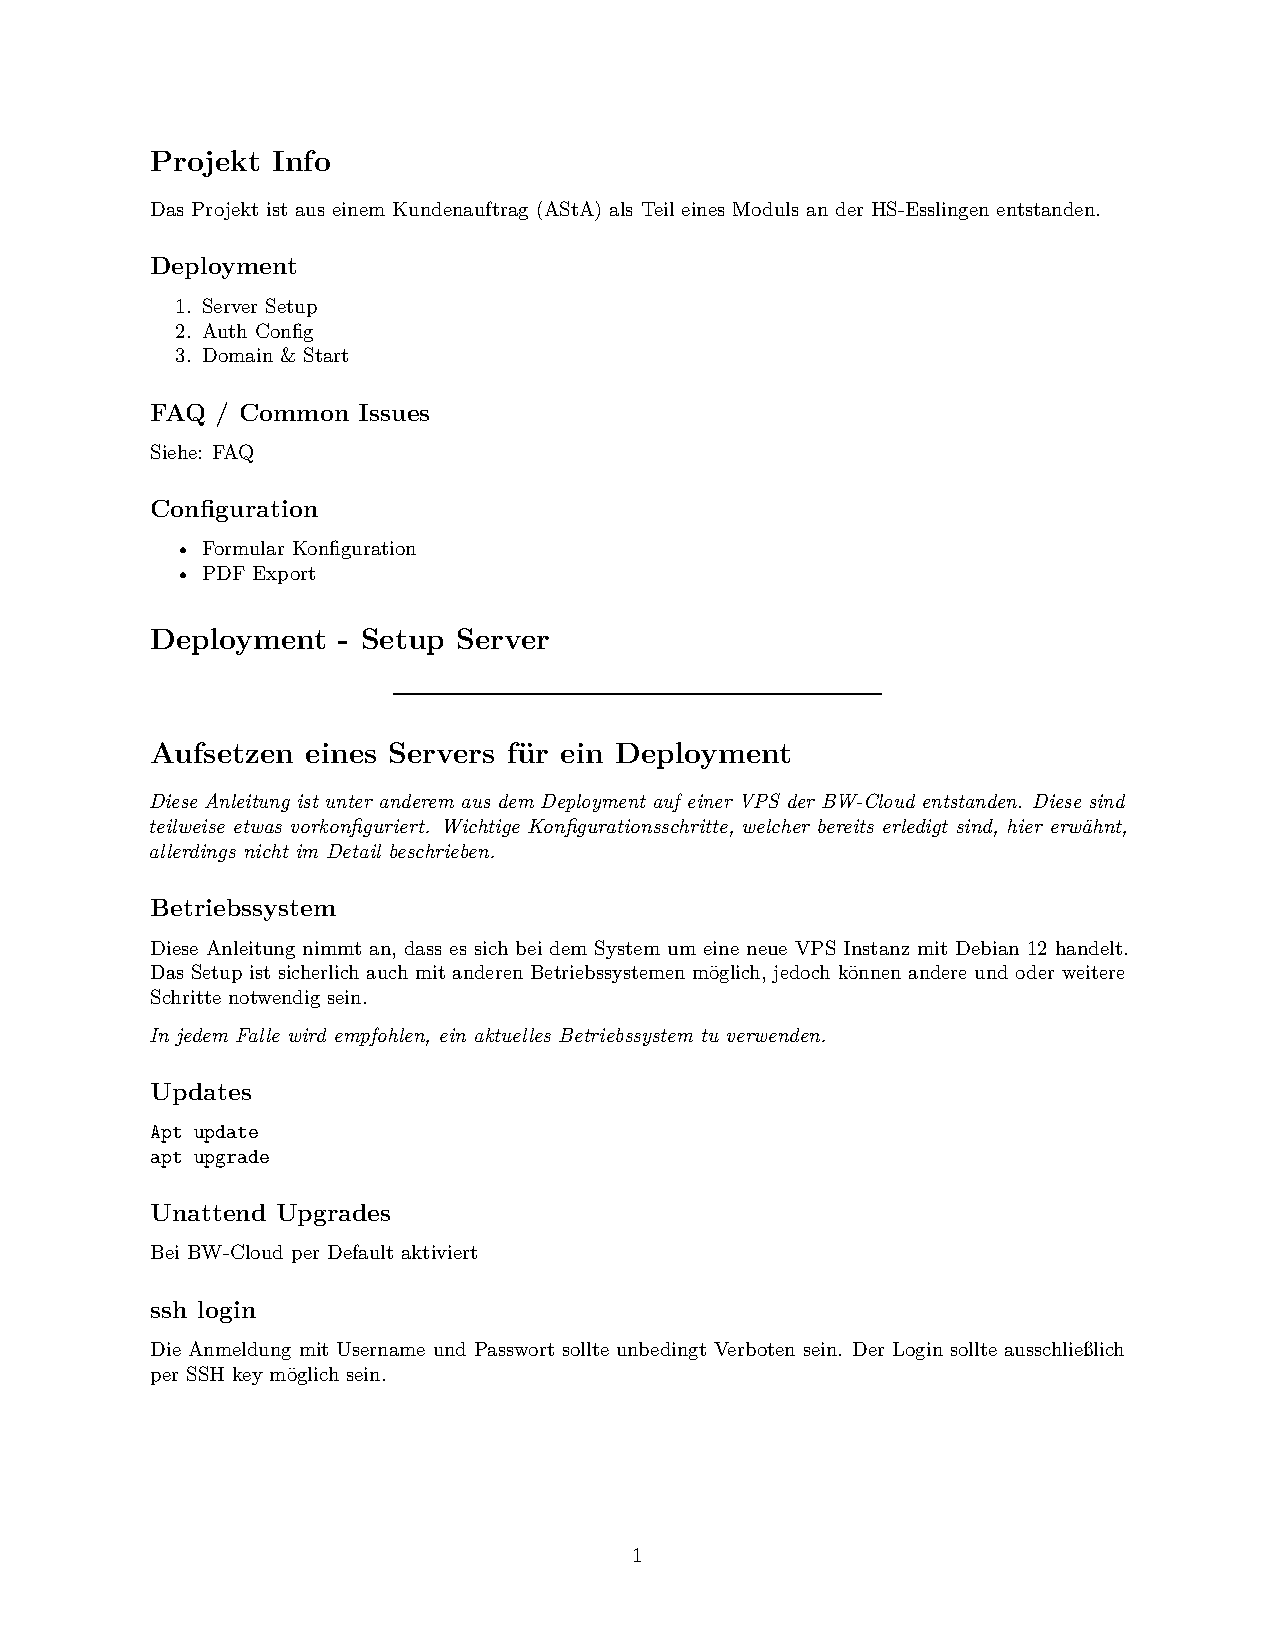
\includepdf[pages=-]{images/guide.pdf}

\section{OpenAPI~Spec}\label{sec:openapi-spec}
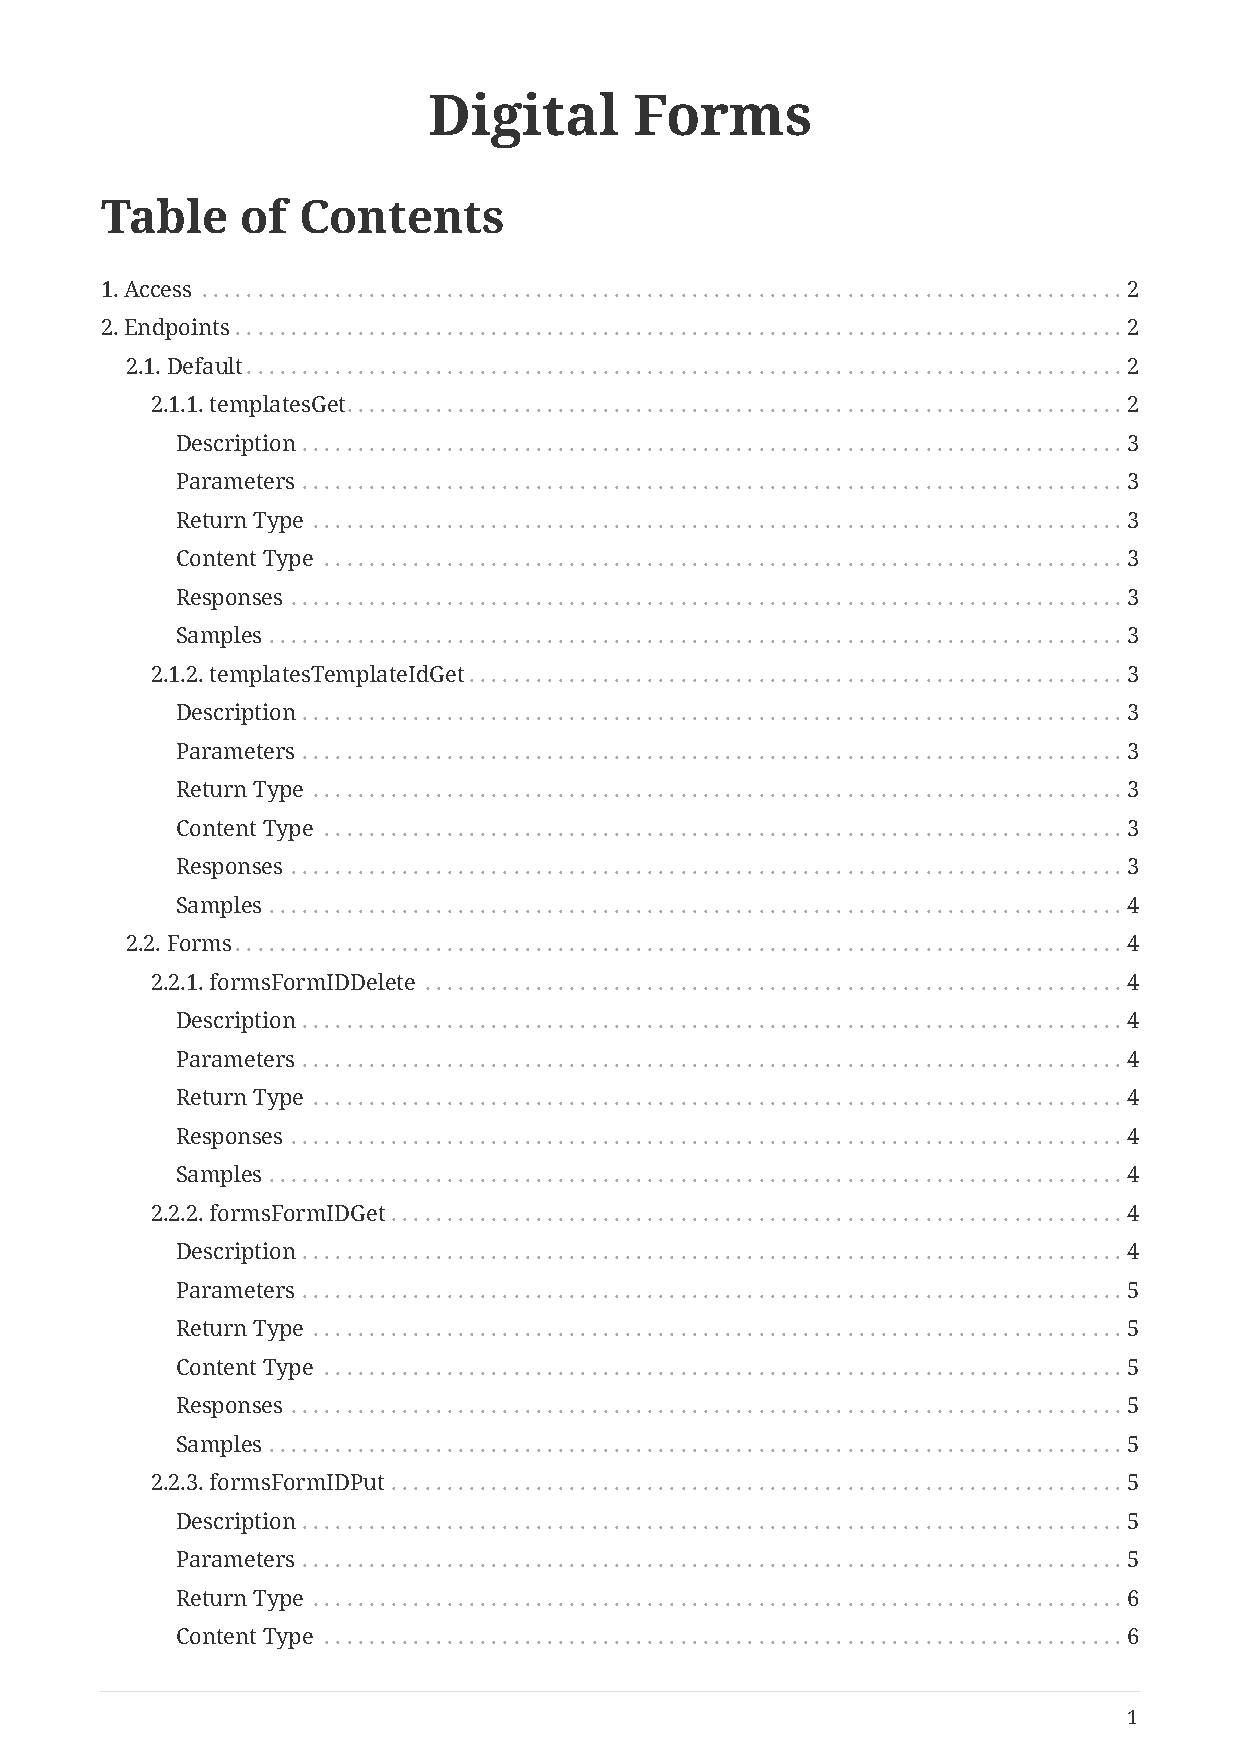
\includepdf[pages=-]{images/API_Spec.pdf}



\section{Backend Abhängigkeitsbaum}\label{sec:backend-abhangigkeitsbaum}
Aufgrund der Länge ausgelagert, erreichbar unter: \url{https://github.com/MaxTrautwein/AStA-Digital-Forms/blob/master/Doc/AnhangAbhaengigkeitsbaum.pdf}

\section{Frontend - Abhängigkeitsbaum}\label{sec:frontend---abhangigkeitsbaum}
Aufgrund der Länge ausgelagert, erreichbar unter: \url{https://github.com/MaxTrautwein/AStA-Digital-Forms/blob/master/Doc/AnhangAbhaengigkeitsbaum.pdf}


\end{document}
